\documentclass[12pt,a4paper]{article}

\usepackage[utf8]{inputenc}
\usepackage[german]{babel}
\usepackage{graphicx}
\usepackage{caption}
\usepackage{subcaption}
\usepackage{float}
\usepackage{booktabs}
\usepackage{csquotes}
\usepackage{hyperref}

%% Math
\usepackage{siunitx}
\usepackage{amsmath}
\usepackage{amssymb}
\graphicspath{
    {../Images/}
}
\begin{document}
	\section{Part 1: Polarisationsgrad}
	Zur Untersuchung des Polarisationsgrades wurden zunächst
	für je beide Detektoren, von Alice als auch von
	Bob, die Zählraten in Abhängigkeit des Polarisationswinkels
	aufgenommen. Hierbei wurde zunächst nicht für koinzidenze Ereignisse
	gefiltert und der Kontrast
	\begin{equation}
		V = \frac{N_{max} - N_{min}}{N_{max} + N_{min}} \label{eq:1}
	\end{equation}
	berechnet.

	Idealerweise, sollte dieser Wert, im ungefilterten Fall, nahe \(0\) sein,
	da die linear senkrecht bzw. horizontal polarisierten Photonen gleichmäßig auf beide Detektorarme verteilt sind
	und die \(\frac{\lambda}{2}\)-Plättchen die Polarisationsrichtung lediglich drehen und keine Photonen absorbieren.
	\newline

	Die Ergebnisse des Kontrasts für die jeweiligen Detektoren sind in Tabelle \ref{tab:ZählratenOhneKoinz} zusammengefasst.
	Hier ist erkennbar das vor allem der Detektor \textbf{A1} einen hohen Kontrast aufweist, dies weist unter anderem
	auf eine nicht perfekte Ausrichtung des optischen Aufbaus hin.
	\begin{table}[H]
		\caption{Kontrast \(V\) - Zählraten ohne Koinzidenzen}\label{tab:ZählratenOhneKoinz}
		\begin{center}
			\begin{tabular}[c]{l|l|l|l}
				\hline
				\multicolumn{1}{c|}{\textbf{Detektor}} &
				\multicolumn{1}{c|}{\textbf{\(N_{min}\)}} &
				\multicolumn{1}{c|}{\textbf{\(N_{max}\)}} &
				\multicolumn{1}{c}{\textbf{\(V\)}} \\
				\hline
				\textbf{Alice 0} & \(30692 \pm 175\) & \(44354 \pm 211\) & \(0.182 \pm 0.004\) \\
				\textbf{Alice 1} & \(17286 \pm 131\) & \(42458 \pm 206\) & \(0.421 \pm 0.004\) \\
				\textbf{Bob 0}   & \(19412 \pm 139\) & \(30613 \pm 175\) & \(0.224 \pm 0.004\) \\
				\textbf{Bob 1}   & \(27686 \pm 166\) & \(31588 \pm 178\) & \(0.066 \pm 0.004\)\\
				% c & d & e\\

				\hline
			\end{tabular}
		\end{center}
	\end{table}
	Um genauere Aussagen zu treffen sind die Ergebnisse in \ref{fig:Einzelzählraten} grafisch dargestellt.
	Bei einer nicht perfekten optischen Ausrichtung würden wir hier für die Winkelabhängigkeit der Zählraten \(N\)
	einen sinusförmigen Verlauf erwarten, da hierdurch eine Tendenz zu vertikal bzw. senkrecht polarisierten Photonen
	zu erwarten sei.
	\newline
	In den Ergebnissen sehen wir eine reine sinusförmige Abhängigkeit jedoch nur für \textbf{A1}, bei den anderen
	Detektoren ist diese nur in Abschnitten zu erkennen, welche durch
	DC-Offsets getrennt sind.
	Dies deutet darauf hin, das während der Aufnahme der Messreihe kleine Störungen am Aufbau vorlagen wie z.B.
	Stöße an dem optischen Tisch, welche die Ausrichtung der Bauteile permanent verändert haben.
	Dies würde bedeuten, dass der Kontrast Niedriger ausfällt, z.B. lege für \textbf{B1} ein Wert von
	\(V=0.15\) vor.
	\newline
	Da diese Vermutung jedoch nur durch weitere Untersuchungen bestätigt werden kann, werden für weitere Vergleiche
	die über die gesamte Messreihe berechneten Kontraste verwendet aus \ref{tab:ZählratenOhneKoinz}.

	\newline



	% \begin{itemize}
	% 	\item   kontrast zwischen max und min
	% 	\item   Kontrast erwartet als nahe null bei idealem Aufbau
	% 	\begin{itemize}
	% 		\item   Hier: B0 A0 hoher kontrast A1 sehr hoher kontrast
	% 		\item 	B1 Hinreichend klein good
	% 		\item 	Sinusodial form spricht für nicht Optimale Versuchkallibrierung / nicht einwandfreie Optik
	% 		\item 	plötzlicher Sprung durhc externe Änderungen (z.b. hintergrundrauschen mehr/weniger, minimale Störung in dem Aufbau)
	% 		\item 	Kontrast womöglich sinvoller in den gleichbleibenden Bereichen -> dadurch kleiner
	% 	\end{itemize}
	% \end{itemize}




	\begin{figure}[H]
		\centering
		\begin{subfigure}[b]{0.45\textwidth}
			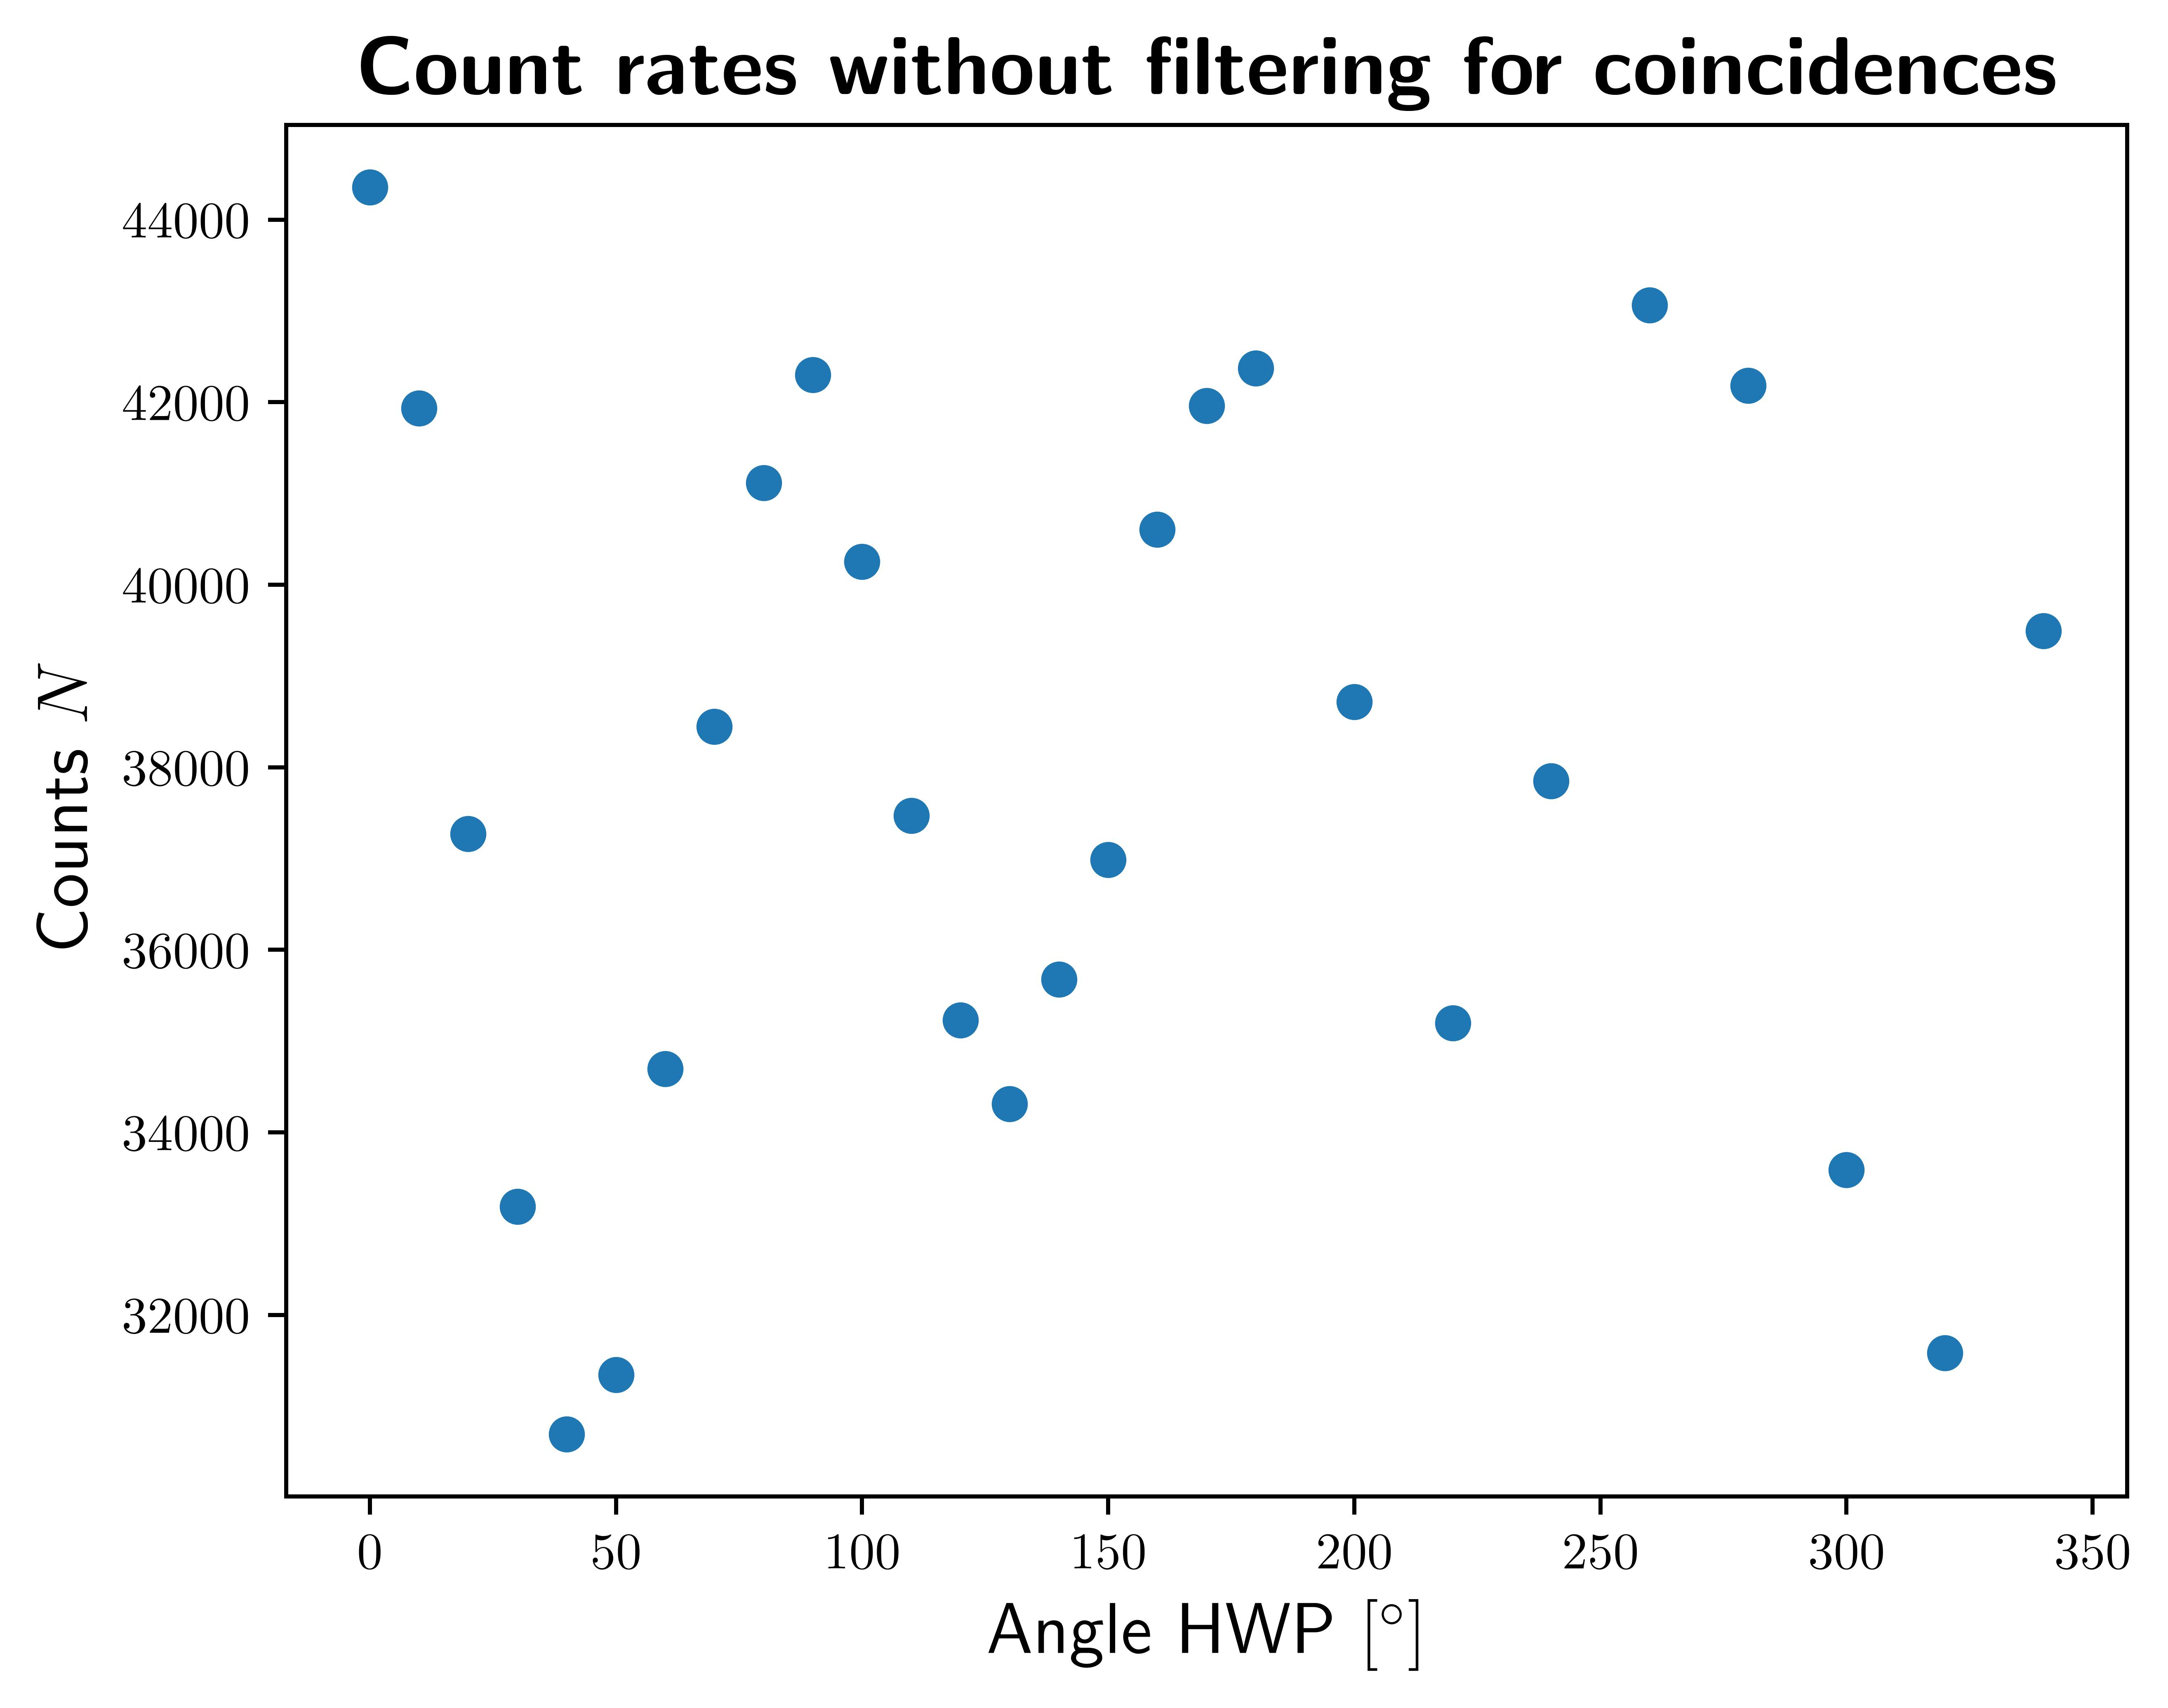
\includegraphics[width=\textwidth]{Einzelzählraten/EinzelzählratenEinzeln_Alice_0.jpg}
			\caption{Alice Detektor 0}
			\label{subfig:A0Einzel}
		\end{subfigure}
		\hfill
		\begin{subfigure}[b]{0.45\textwidth}
			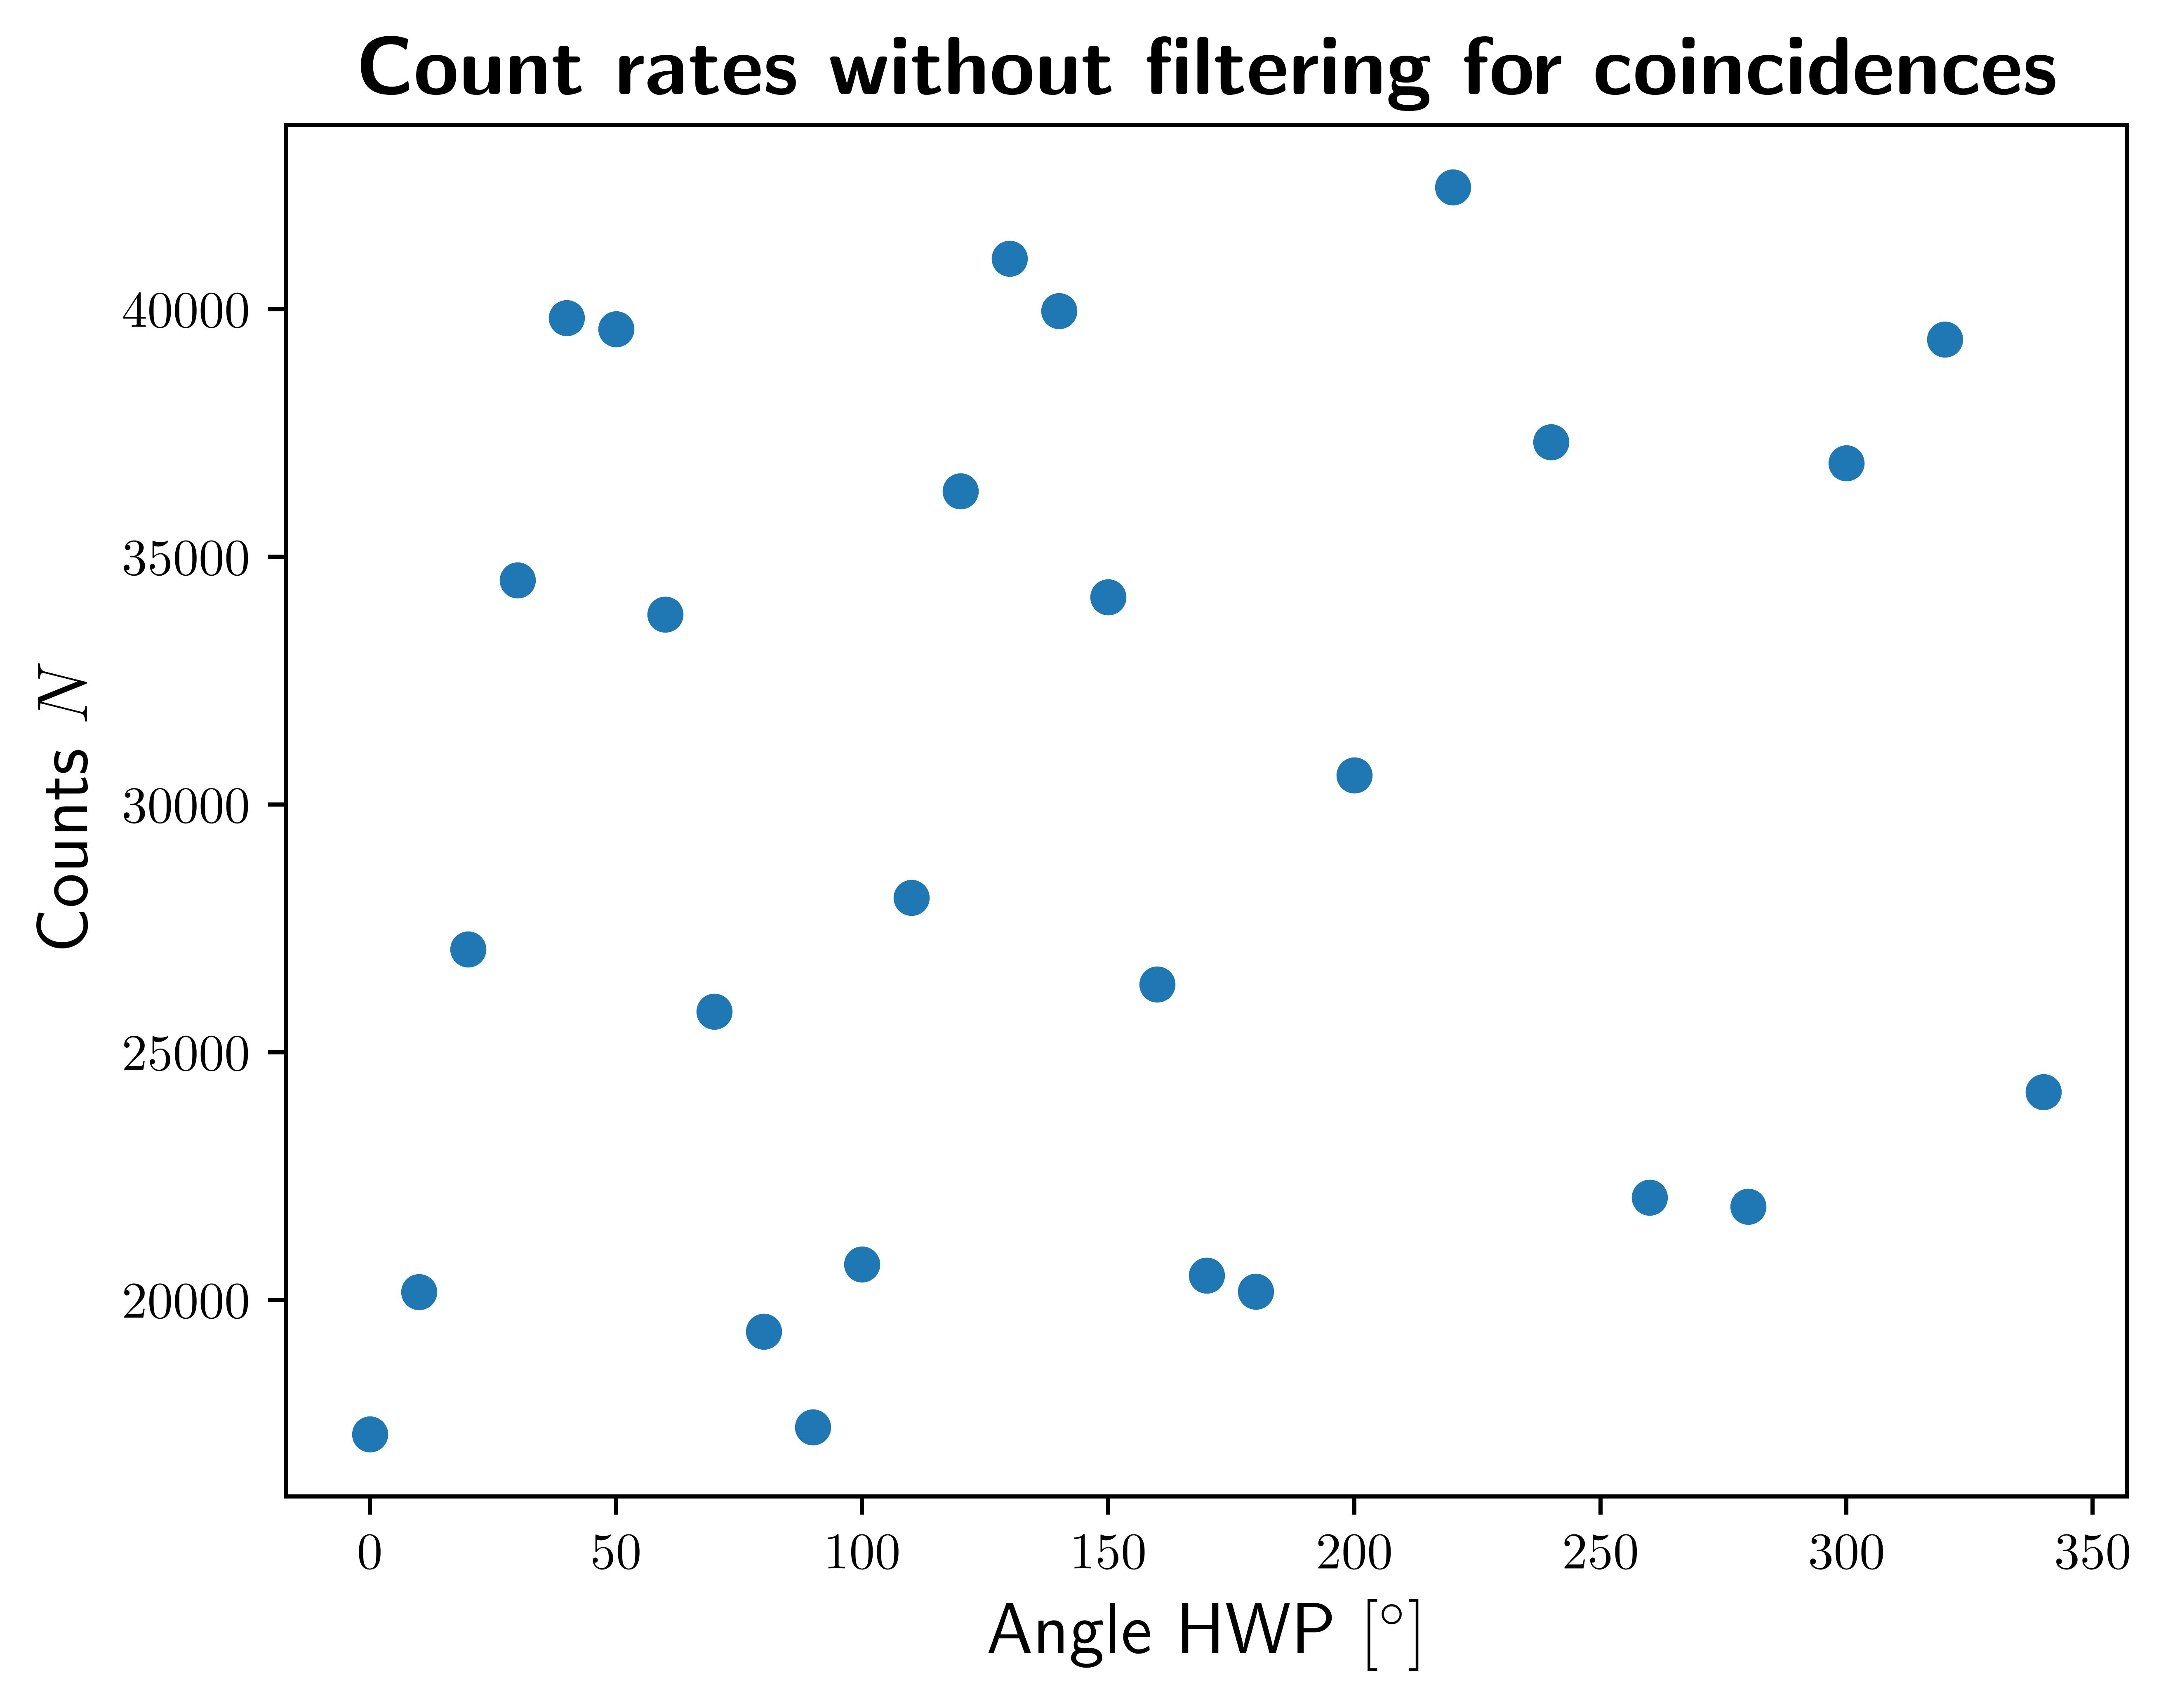
\includegraphics[width=\textwidth]{Einzelzählraten/EinzelzählratenEinzeln_Alice_1.jpg}
			\caption{Alice Detektor 1}
			\label{subfig:A1Eiinzel}
		\end{subfigure}
		\vskip\baselineskip
		\begin{subfigure}[b]{0.45\textwidth}
			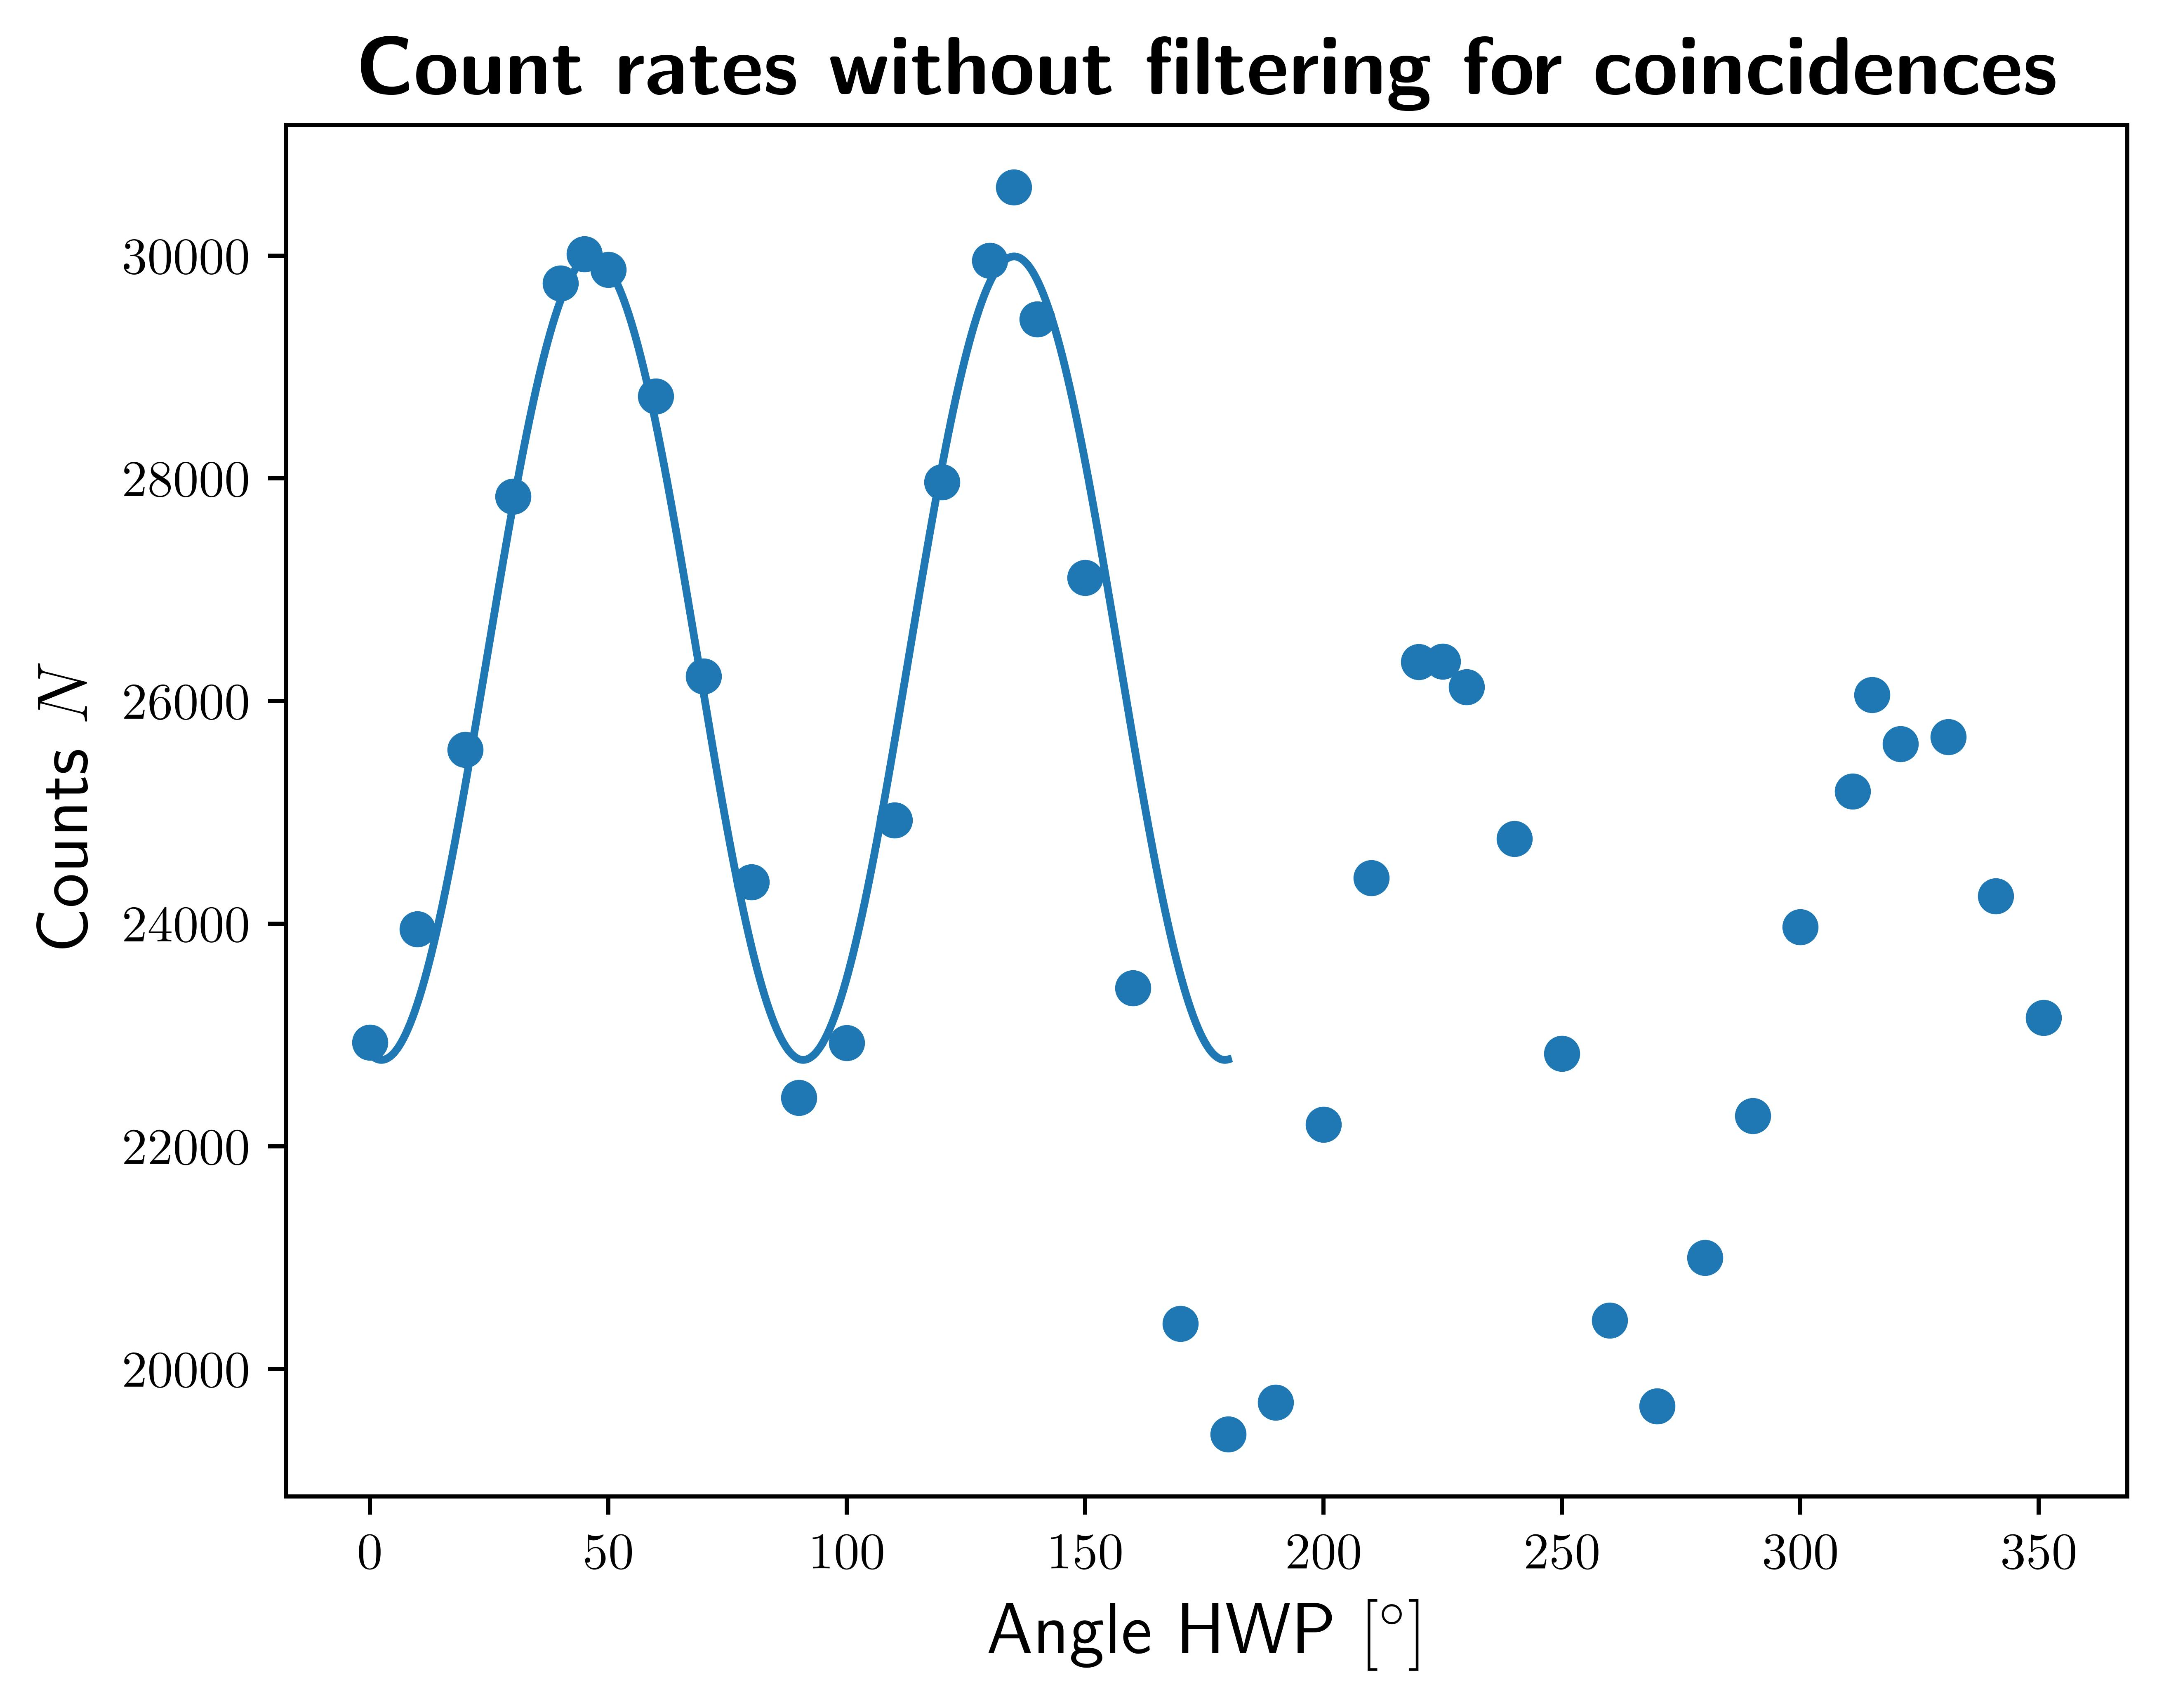
\includegraphics[width=\textwidth]{Einzelzählraten/EinzelzählratenEinzeln_Bob_0.jpg}
			\caption{Bob Detektor 0}
			\label{subfig:B0Einzel}
		\end{subfigure}
		\hfill
		\begin{subfigure}[b]{0.45\textwidth}
			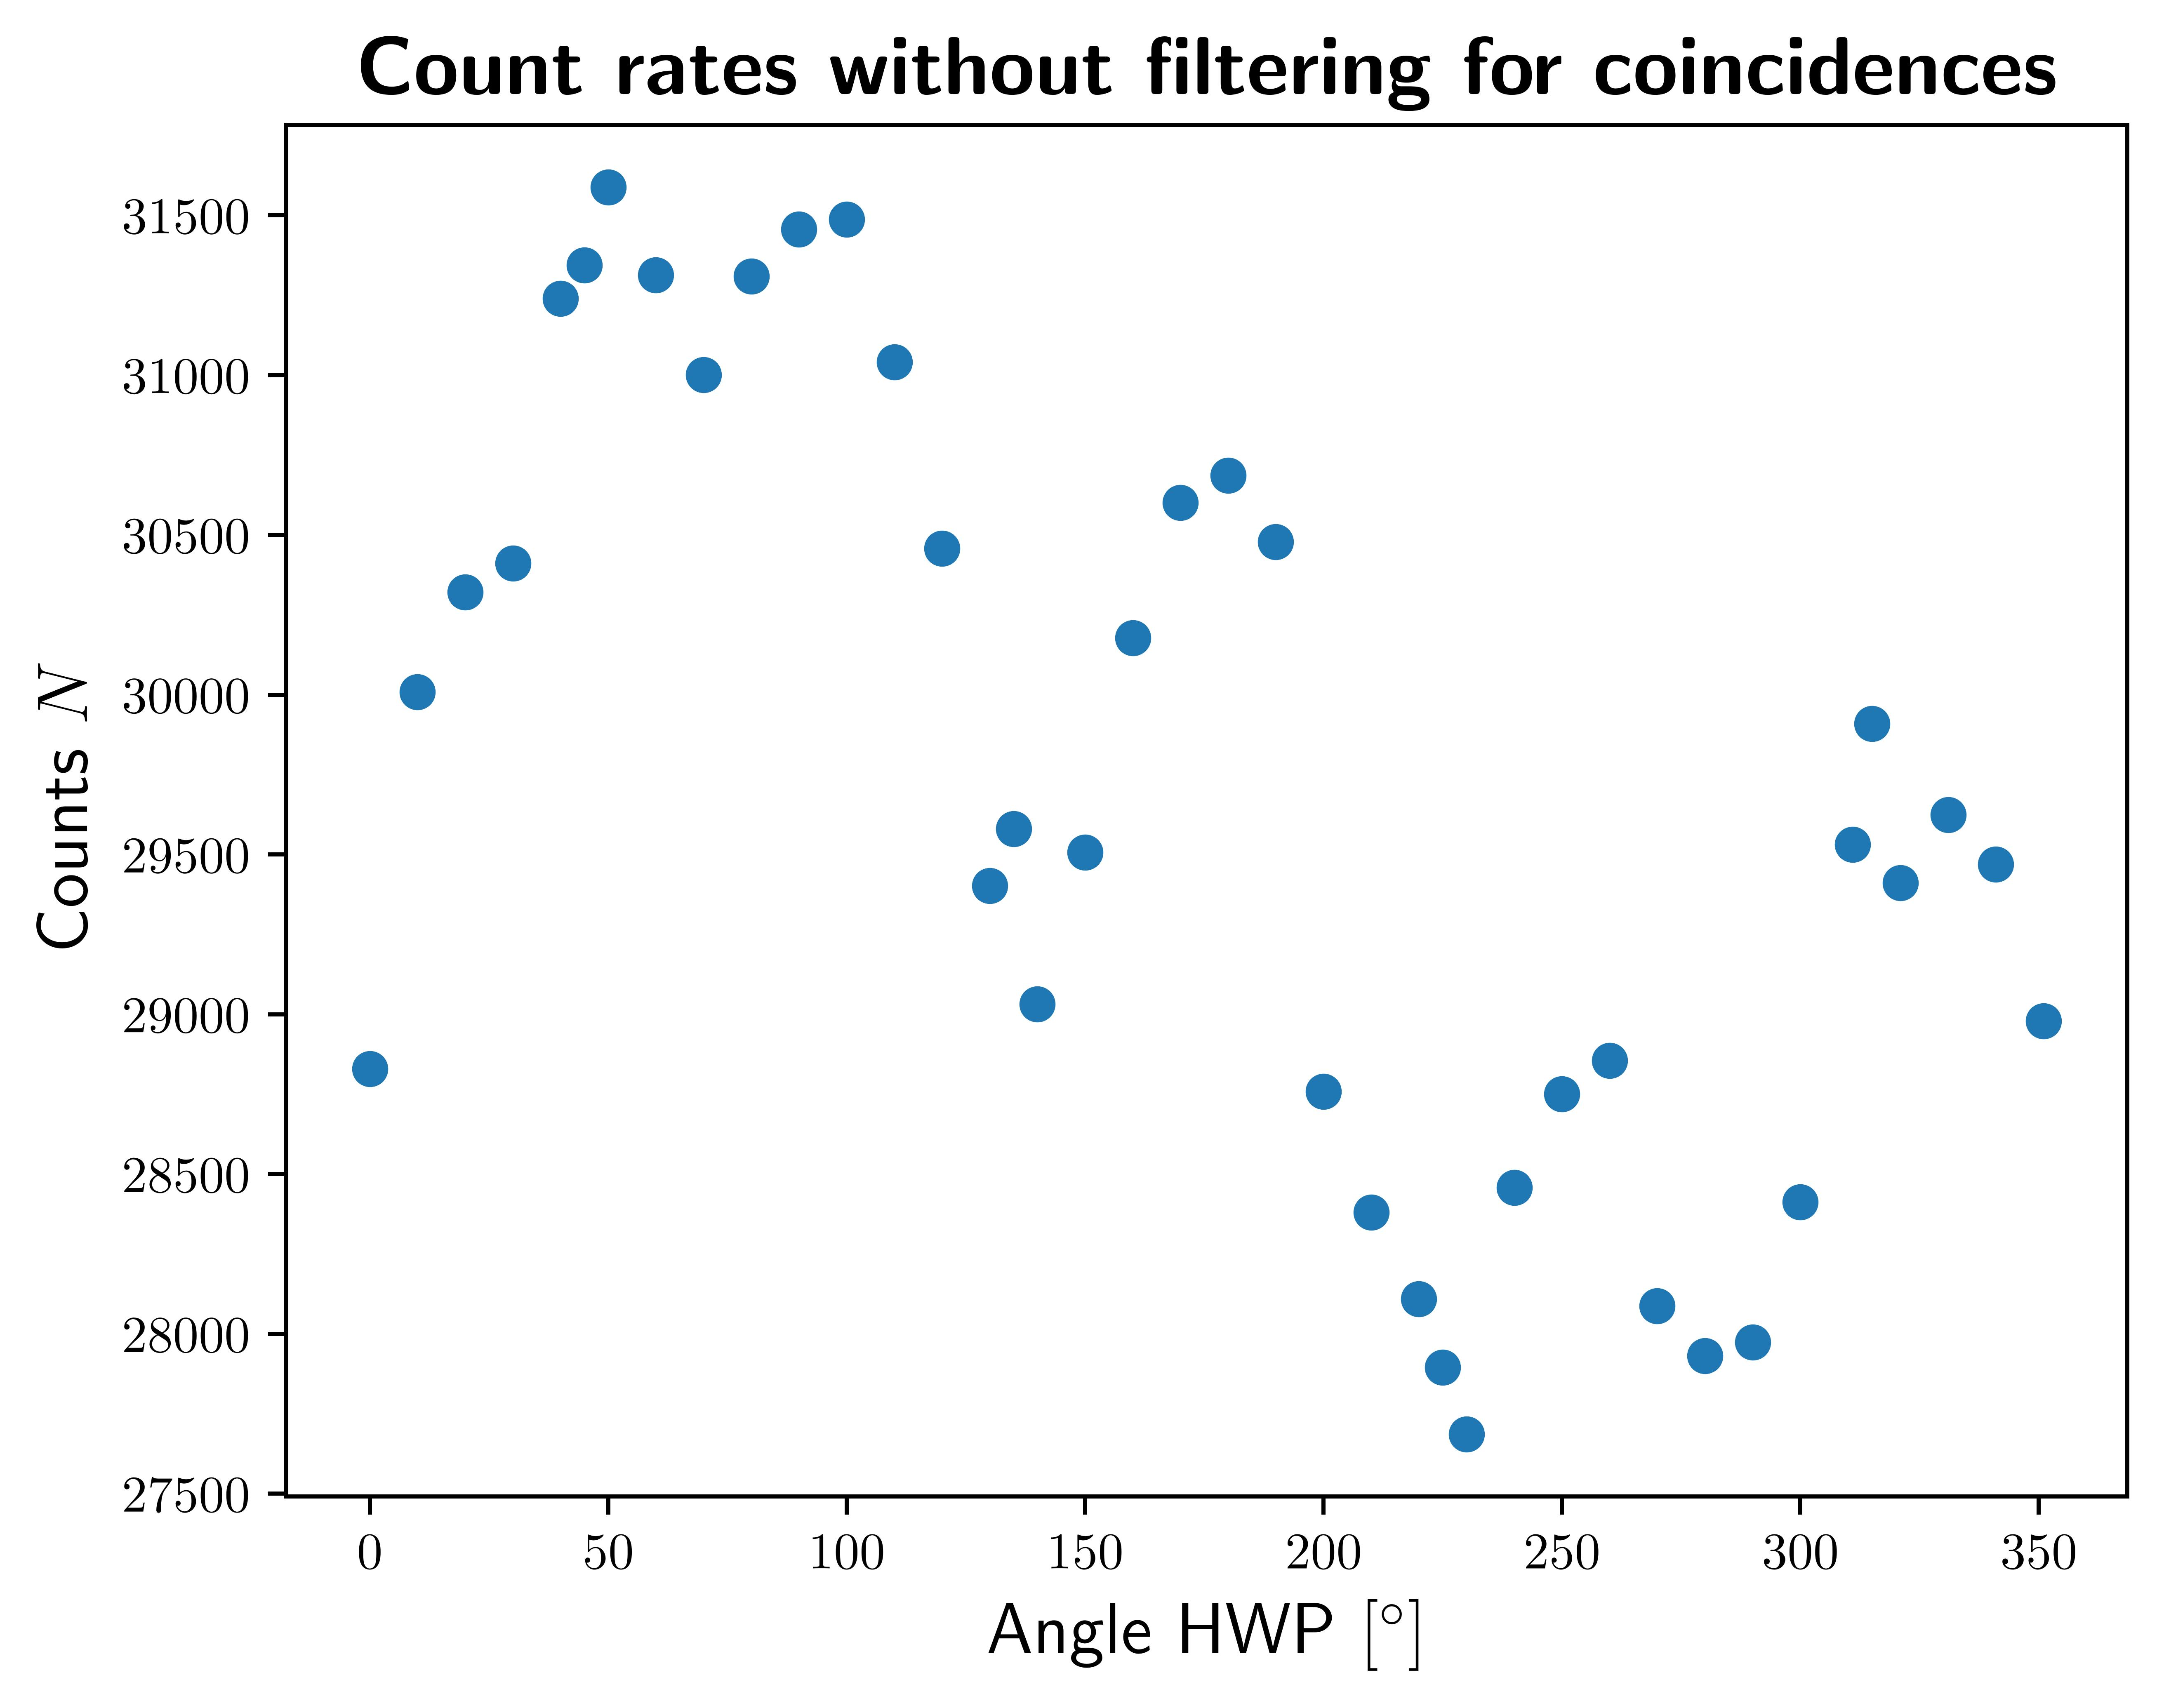
\includegraphics[width=\textwidth]{Einzelzählraten/EinzelzählratenEinzeln_Bob_1.jpg}
			\caption{Bob Detektor 1}
			\label{subfig:B1Einzel}
		\end{subfigure}
		\caption{
    		Einzelzählraten der jeweiligen Detektoren gemessen über 5 Sekunden, ohne Berücksichtigung der Koinzidenzen.
    		Für Detektor B1 wurde ebenfalls der Sinusförmige verlauf der ersten Hälfte dargestellt, welcher
            gerade bei einer nicht perfekten optischen Ausrichtung zu erwarten ist.
		}
		\label{fig:Einzelzählraten}
	\end{figure}


	Im Folgenden soll die Polarisationsabhängigkeit der auf Koinzidenzen gefilterten Zählraten untersucht werden,
	hierfür wird die Polarisation in einem der Arme fixiert und in dem anderen Arm systematisch variiert.
	Es wurden vier Messreihen aufgenommen, hierbei wurden jeweils Alice und Bob
	in der \(0/90^\circ\) und \(-45/+45^\circ\) Basis fixiert und die Ergebnisse in \ref{tab:Koinzidenzen} tabellarisch
	dargestellt.
	Zu beachten war hierbei, dass die Winkel den tatsächlichen Polarisationswinkel beschreiben,
	welcher dem doppelten Winkel des \(\frac{\lambda}{2}\)-Plättchens entsprechen.
	Die Ergebnisse der Messreihe mit Alice fixiert auf in der \(0/90^\circ \) Basis sind
	in \ref{fig:KoinzidenzAlice0/90AlleDetektoren} grafisch dargestellt.
	Hier ist zu erkennen, dass sehr gute Werte mit \(V \geq 0.9\) mit einer deutlich
	höheren maximal Zählrate einhergehen. Dies spricht, wie bei der vorherigen Einzelzählraten Messung
	bereits vermutet, ebenfalls für eine nicht optimale Justierung der Bauteile, da mit einer räumlichen Verschiebung, der
	Detektoren, weg von den Schnittpunkten der Fluoreszenzkegel, die Wahrscheinlichkeit,
	zueinander gehörender verschränkte Photonen an beiden Detektoren zu messen, sinkt.

	% Die gemessenen Ereignisse sind in Graphik~\ref{fig:Einzelzählraten} dargestellt.

	\subsection{Kontrast Koinzidenzen}
	% \begin{itemize}
	% 	\item   Kontraste sehr gut bis gut für 0 als auch 45 Grad
	% 	\item 	schlechtester Wert ca. 0.71, nicht gut
	% 	\item
	% \end{itemize}

	\begin{table}[H]
	\label{tab:Koinzidenzen}
	\caption{
	Auf Koinzidenzen gefilterte min und max Zählraten, sowie der Kontrast berechnet nach \ref{eq:1}.
	Jeweils für Alice und Bob fixierte Basis auf \(0/90^\circ\) bzw. \(\pm 45^\circ\).
	Abgesehen von zwei Ausreißern in \ref{tab:ZählratenMitKoinzFixAlice} und \ref{tab:ZählratenMitKoinzFixBob45}, sind Werte größer
	als 0.8 zu sehen. Die Diskrepanz zu dem Idealwert von \(1\) sind unter anderem auf eine nicht
	ideale Ausrichtung der optischen Apparaturen zurückzuführen.
	}
	\centering
		\begin{subtable}[b]{0.45\textwidth}
    		\caption{Kontrast \(V\) - Zählraten mit Berücksichtigung von Koinzidenzen Basis \(0/90^\circ\), Fixiert Alice}\label{tab:ZählratenMitKoinzFixAlice}
    		\begin{center}
                \resizebox{1.1\linewidth}{!}{
    			\begin{tabular}[c]{l|l|l|l}
    				\hline
    				\multicolumn{1}{c|}{\textbf{Detektor}} &
    				\multicolumn{1}{c|}{\textbf{\(N_{min}\)}} &
    				\multicolumn{1}{c|}{\textbf{\(N_{max}\)}} &
    				\multicolumn{1}{c}{\textbf{\(V\)}} \\
    				\hline
    				\textbf{A0B0} & \(30 \pm 5\)      & \(979 \pm 31\)   & \(0.941 \pm 0.028\) \\
    				\textbf{A0B1} & \(32 \pm 6\)      & \(1122 \pm 33\)  & \(0.945 \pm 0.013\) \\
    				\textbf{A1B0} & \(17 \pm 4\)      & \(101 \pm 10\)   & \(0.71 \pm 0.04\)   \\
    				\textbf{A1B1} & \(13 \pm 4\)      & \(129 \pm 11\)   & \(0.817 \pm 0.015\) \\
    				% c & d & e\\
    				\hline
    			\end{tabular}}
    		\end{center}
    	\end{subtable}
		\hfill
		\begin{subtable}[b]{0.45\textwidth}
          		\caption{Kontrast \(V\) - Zählraten mit Berücksichtigung von Koinzidenzen Basis \(0/90^\circ\), Fixiert Bob}\label{tab:ZählratenMitKoinzFixBob90}
          		\begin{center}
                \resizebox{1.1\linewidth}{!}{
         			\begin{tabular}[c]{l|l|l|l}
            				\hline
            				\multicolumn{1}{c|}{\textbf{Detektor}} &
            				\multicolumn{1}{c|}{\textbf{\(N_{min}\)}} &
            				\multicolumn{1}{c|}{\textbf{\(N_{max}\)}} &
            				\multicolumn{1}{c}{\textbf{\(V\)}} \\
            				\hline
            				\textbf{A0B0} & \(30 \pm 5\)      & \(346 \pm 19\)   & \(0.840 \pm 0.028\) \\
            				\textbf{A0B1} & \(51 \pm 7\)      & \(1021 \pm 32\)  & \(0.905 \pm 0.013\) \\
            				\textbf{A1B0} & \(8 \pm 2.9\)     & \(114 \pm 11\)   & \(0.87 \pm 0.04\)   \\
            				\textbf{A1B1} & \(22 \pm 4.7\)    & \(605 \pm 25\)   & \(0.930 \pm 0.015\) \\
            				% c & d & e\\

            				\hline
         			\end{tabular}}
          		\end{center}
		\end{subtable}
		\vskip\baselineskip
		\begin{subtable}[b]{0.45\textwidth}
          		\caption{Kontrast \(V\) - Zählraten mit Berücksichtigung von Koinzidenzen Basis \(\pm 45^\circ\), fixiert Bob}\label{tab:ZählratenMitKoinzFixBob45}
          		\begin{center}
            \resizebox{1.1\linewidth}{!}{
         			\begin{tabular}[c]{l|l|l|l}
            				\hline
            				\multicolumn{1}{c|}{\textbf{Detektor}} &
            				\multicolumn{1}{c|}{\textbf{\(N_{min}\)}} &
            				\multicolumn{1}{c|}{\textbf{\(N_{max}\)}} &
            				\multicolumn{1}{c}{\textbf{\(V\)}} \\
            				\hline
            				\textbf{A0B0} & \(71 \pm 8\)      & \(492 \pm 22\)   & \(0.748 \pm 0.028\) \\
            				\textbf{A0B1} & \(39 \pm 6\)      & \(738 \pm 27\)   & \(0.900 \pm 0.016\) \\
            				\textbf{A1B0} & \(16 \pm 4\)      & \(272 \pm 16\)   & \(0.889 \pm 0.027\) \\
            				\textbf{A1B1} & \(33 \pm 6\)      & \(359 \pm 19\)   & \(0.831 \pm 0.028\) \\
            				% c & d & e\\

            				\hline
         			\end{tabular}}
          		\end{center}
		\end{subtable}
		\hfill
		\begin{subtable}[b]{0.45\textwidth}
          		\caption{Kontrast \(V\) - Zählraten mit Berücksichtigung von Koinzidenzen Basis \(\pm 45^\circ\), fixiert Alice}\label{tab:ZählratenMitKoinzFixAlice45}
          		\begin{center}
            \resizebox{1.1\linewidth}{!}{
         			\begin{tabular}[c]{l|l|l|l}
            				\hline
            				\multicolumn{1}{c|}{\textbf{Detektor}} &
            				\multicolumn{1}{c|}{\textbf{\(N_{min}\)}} &
            				\multicolumn{1}{c|}{\textbf{\(N_{max}\)}} &
            				\multicolumn{1}{c}{\textbf{\(V\)}} \\
            				\hline
            				\textbf{A0B0} & \(43 \pm 7\)      & \(465 \pm 22\)   & \(0.831 \pm 0.025\) \\
            				\textbf{A0B1} & \(55 \pm 7\)      & \(540 \pm 23\)   & \(0.815 \pm 0.024\) \\
            				\textbf{A1B0} & \(20 \pm 4\)      & \(363 \pm 19\)   & \(0.896 \pm 0.023\) \\
            				\textbf{A1B1} & \(25 \pm 5\)      & \(423 \pm 21\)   & \(0.888 \pm 0.022\) \\
            				% c & d & e\\

            				\hline
         			\end{tabular}}
          		\end{center}
		\end{subtable}
	\end{table}

	\begin{figure}[H]
		\centering
		\begin{subfigure}[b]{0.45\textwidth}
			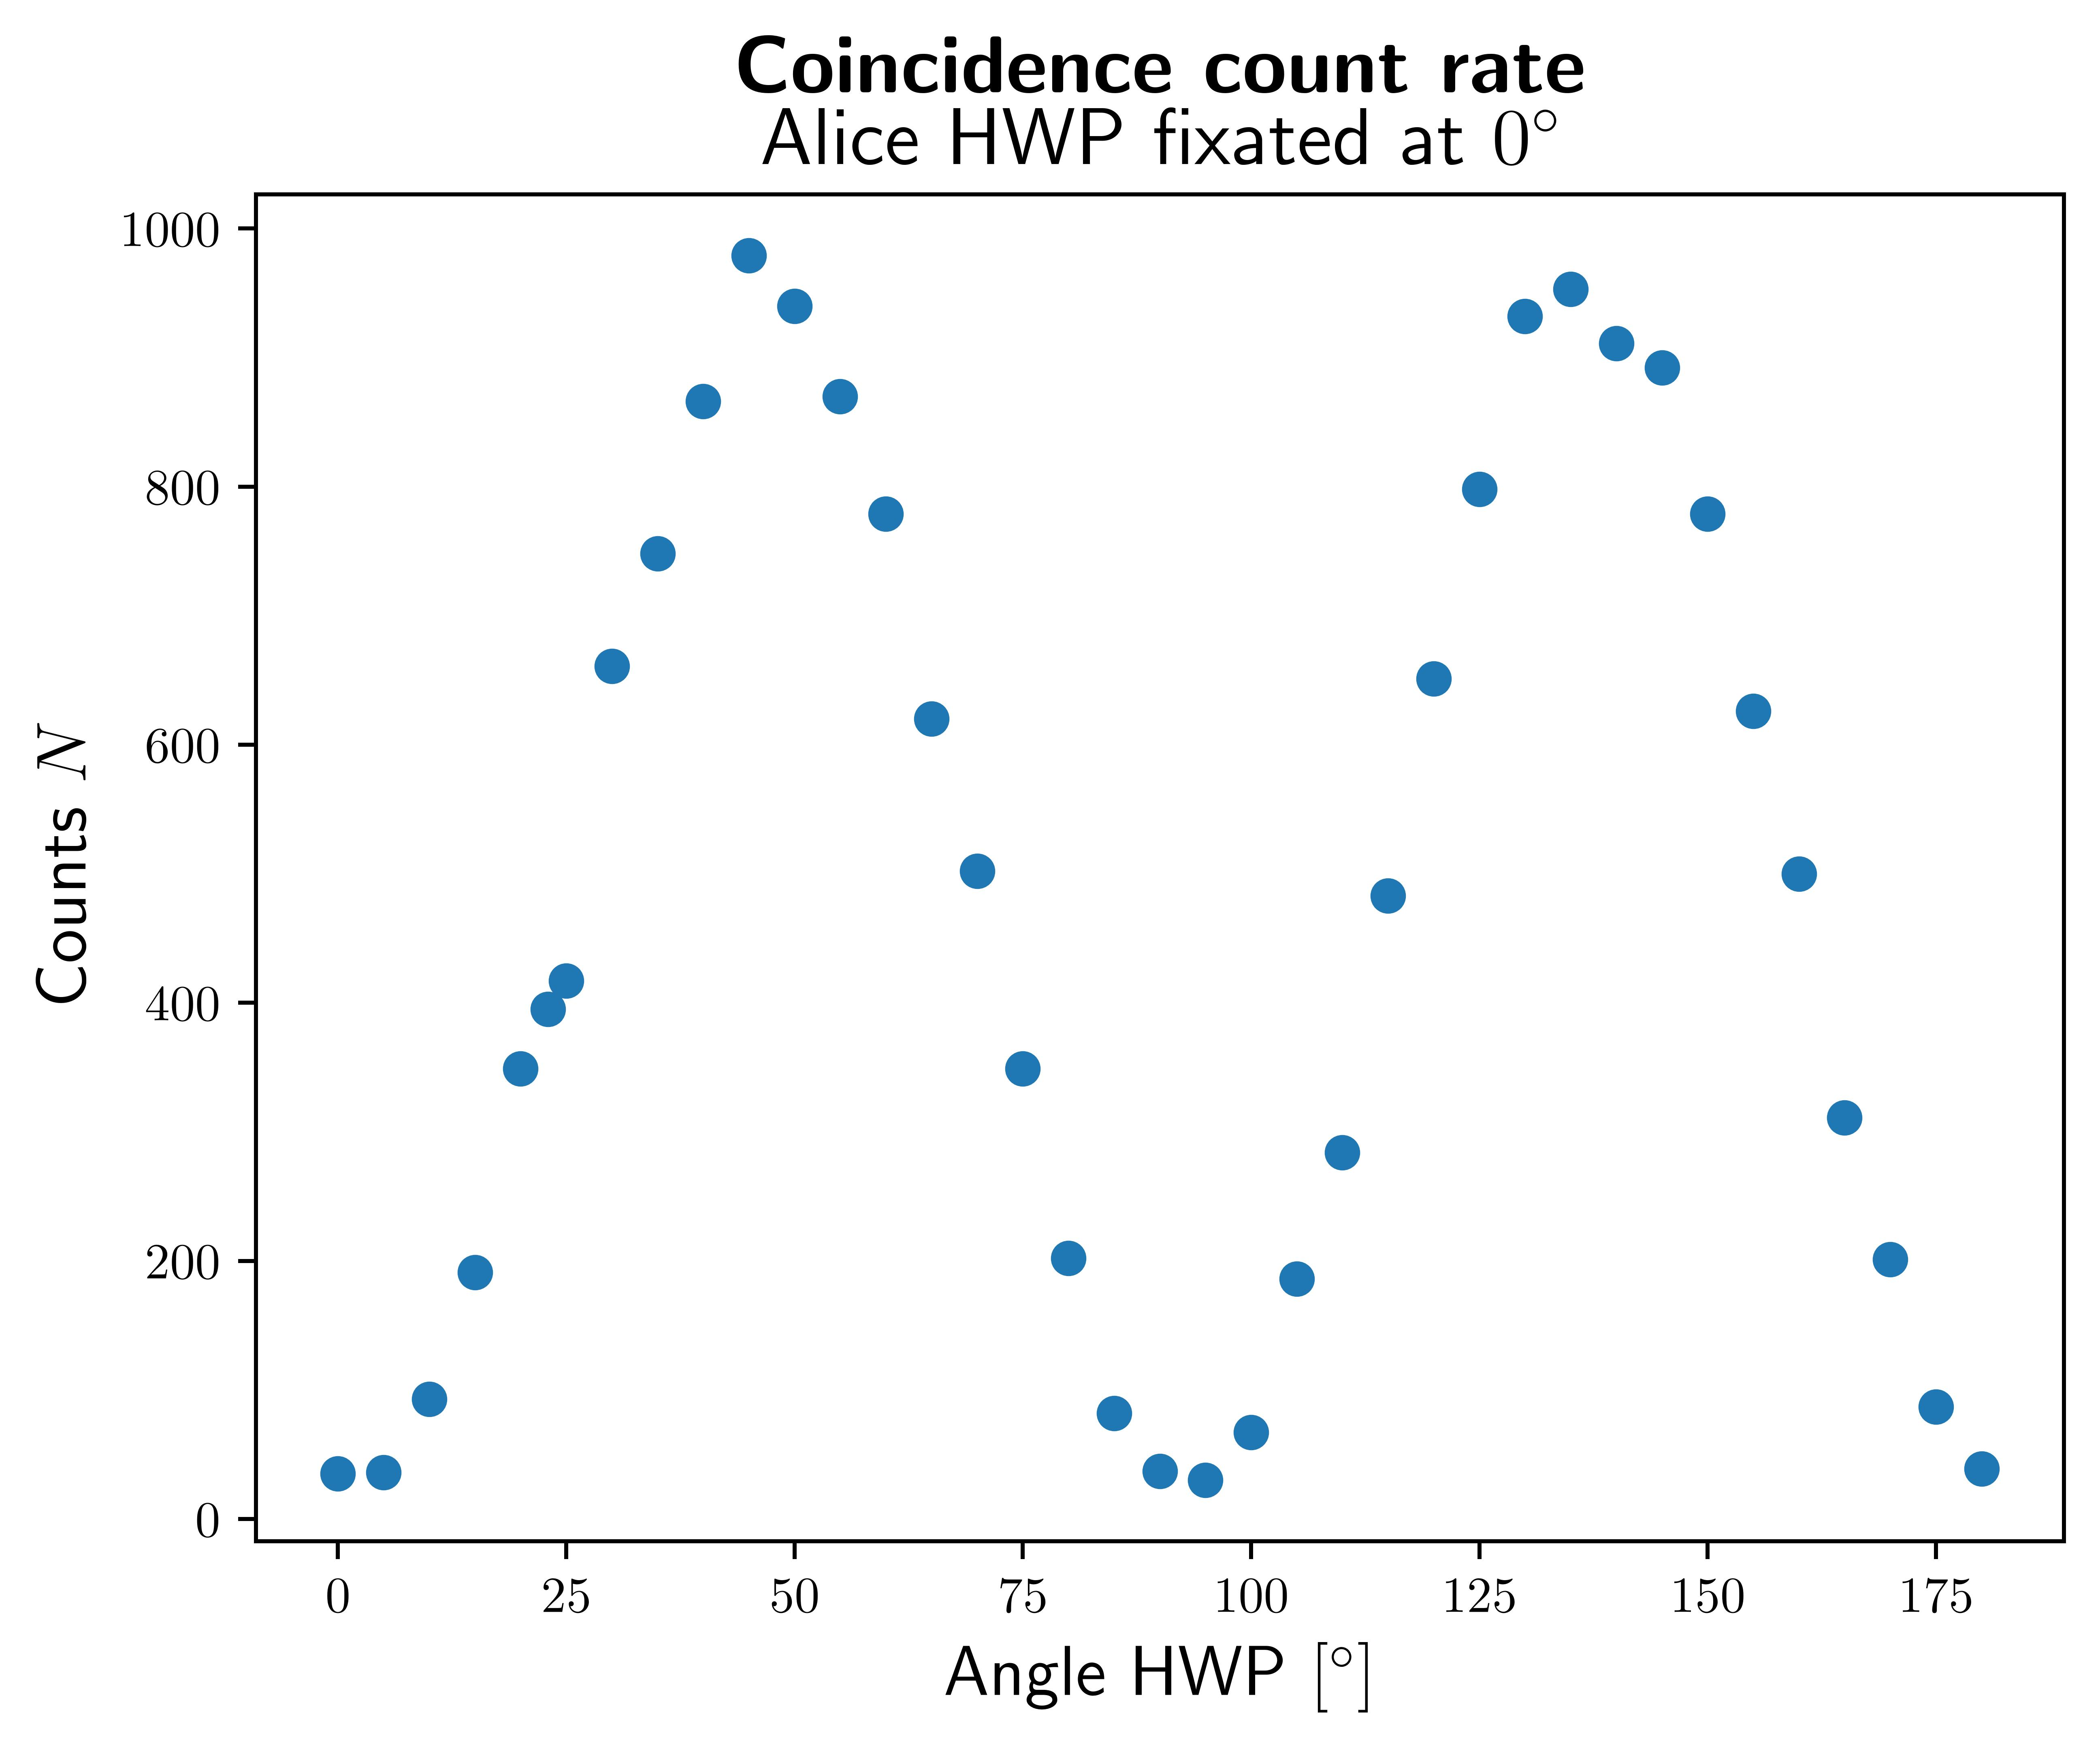
\includegraphics[width=\textwidth]{Koinzidenz/KoinzidenztählratenAliceFixiert0_90_A0B0.jpg}
			\caption{Detektors A0B0}
			\label{fig:A0B0Alice0/90}
		\end{subfigure}
		\hfill
		\begin{subfigure}[b]{0.45\textwidth}
			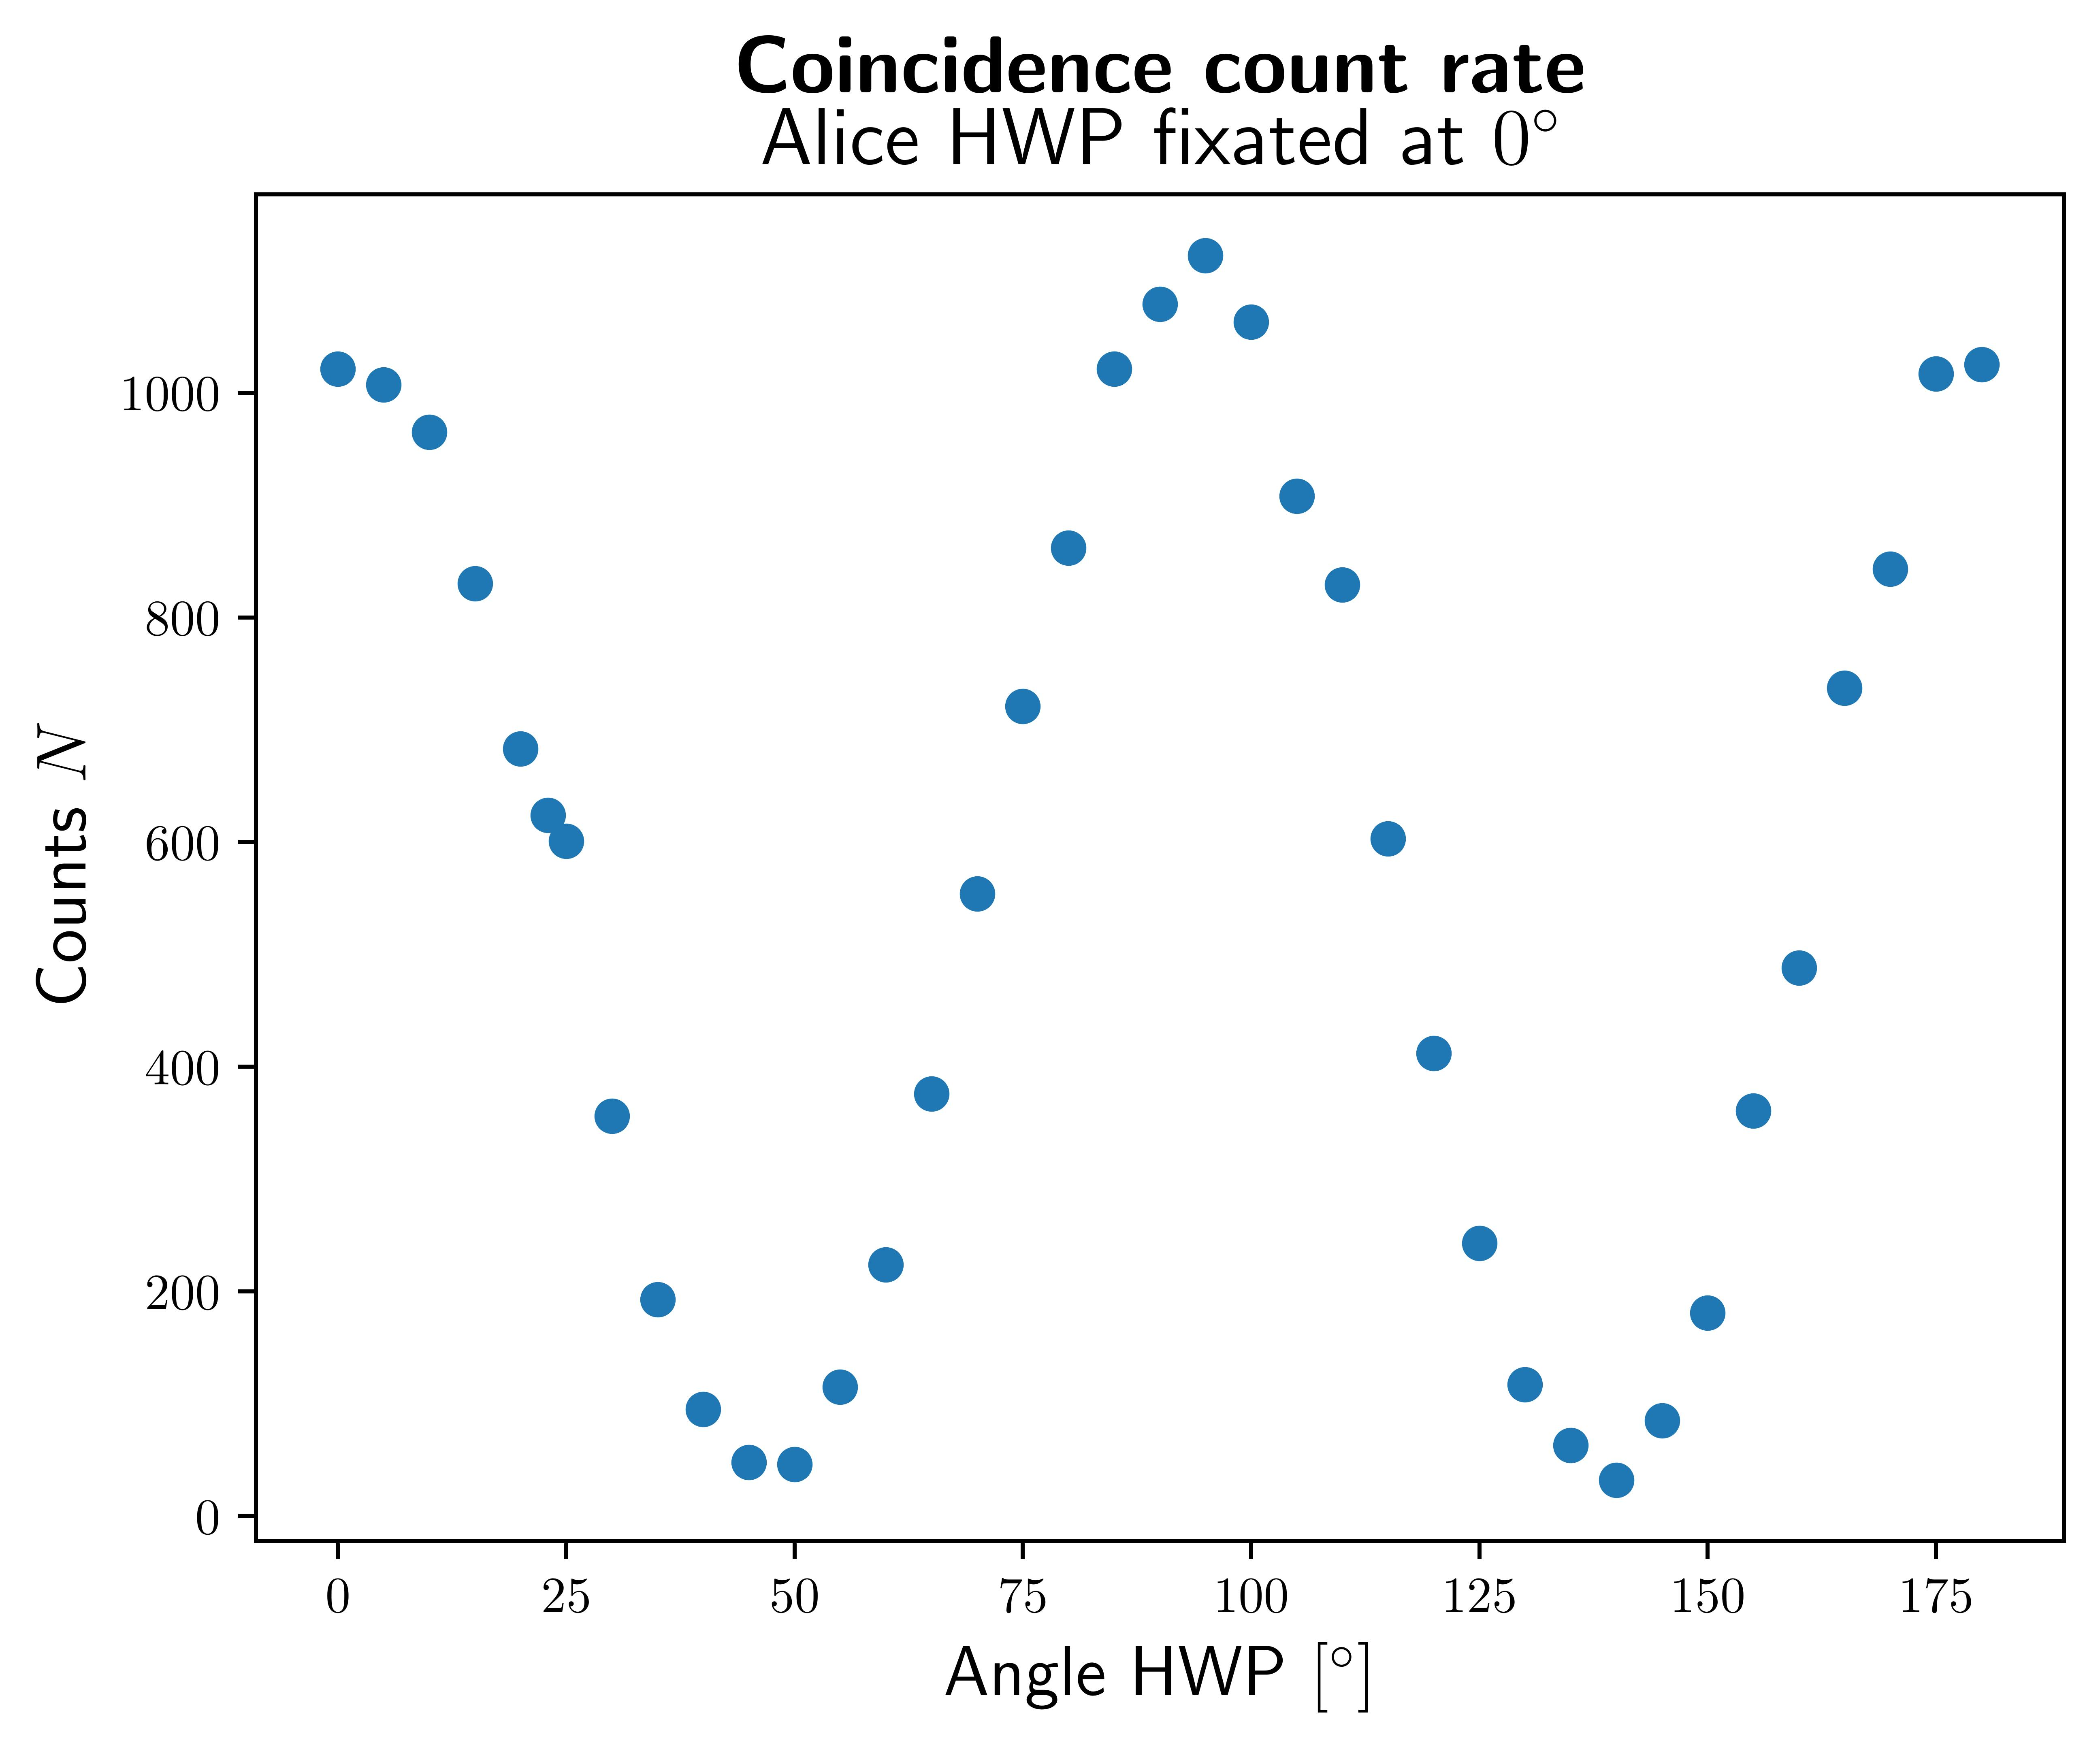
\includegraphics[width=\textwidth]{Koinzidenz/KoinzidenztählratenAliceFixiert0_90_A0B1.jpg}
			\caption{Detektors A0B1}
			\label{fig:A0B1Alice0/90}
		\end{subfigure}
		\vskip\baselineskip
		\begin{subfigure}[b]{0.45\textwidth}
			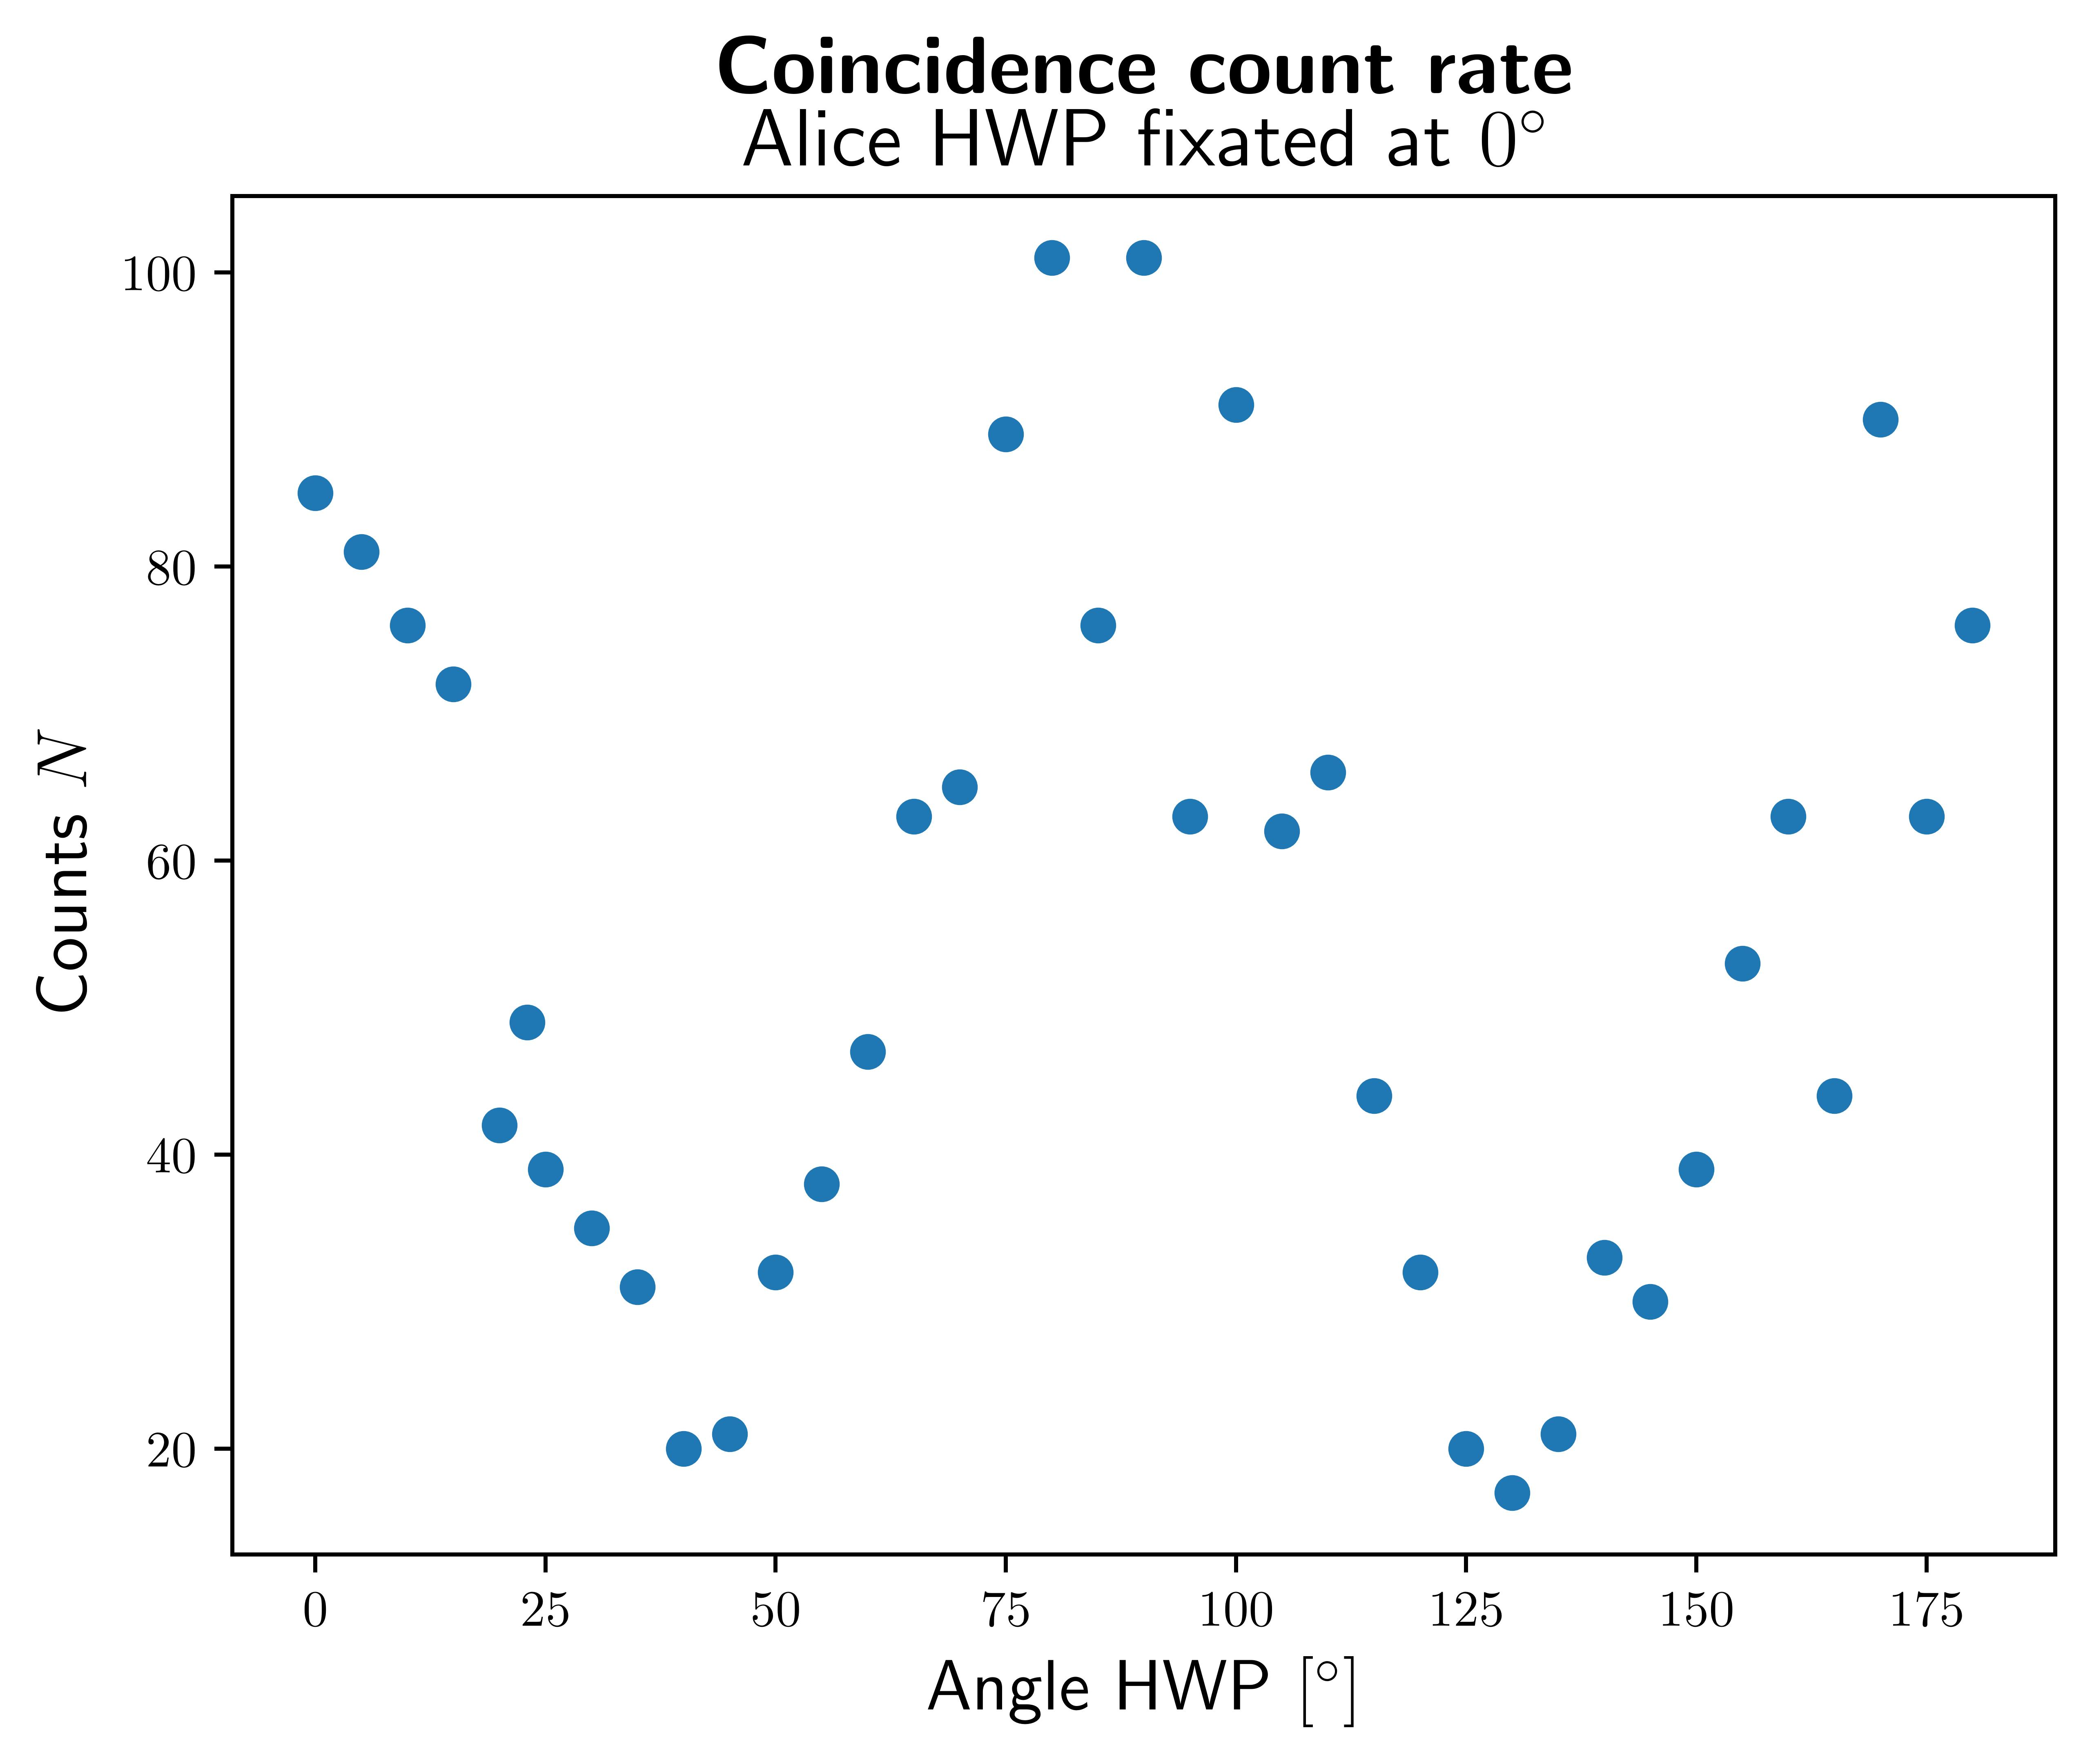
\includegraphics[width=\textwidth]{Koinzidenz/KoinzidenztählratenAliceFixiert0_90_A1B0.jpg}
			\caption{Detektors A1B0}
			\label{fig:A1B0}
		\end{subfigure}
		\hfill
		\begin{subfigure}[b]{0.45\textwidth}
			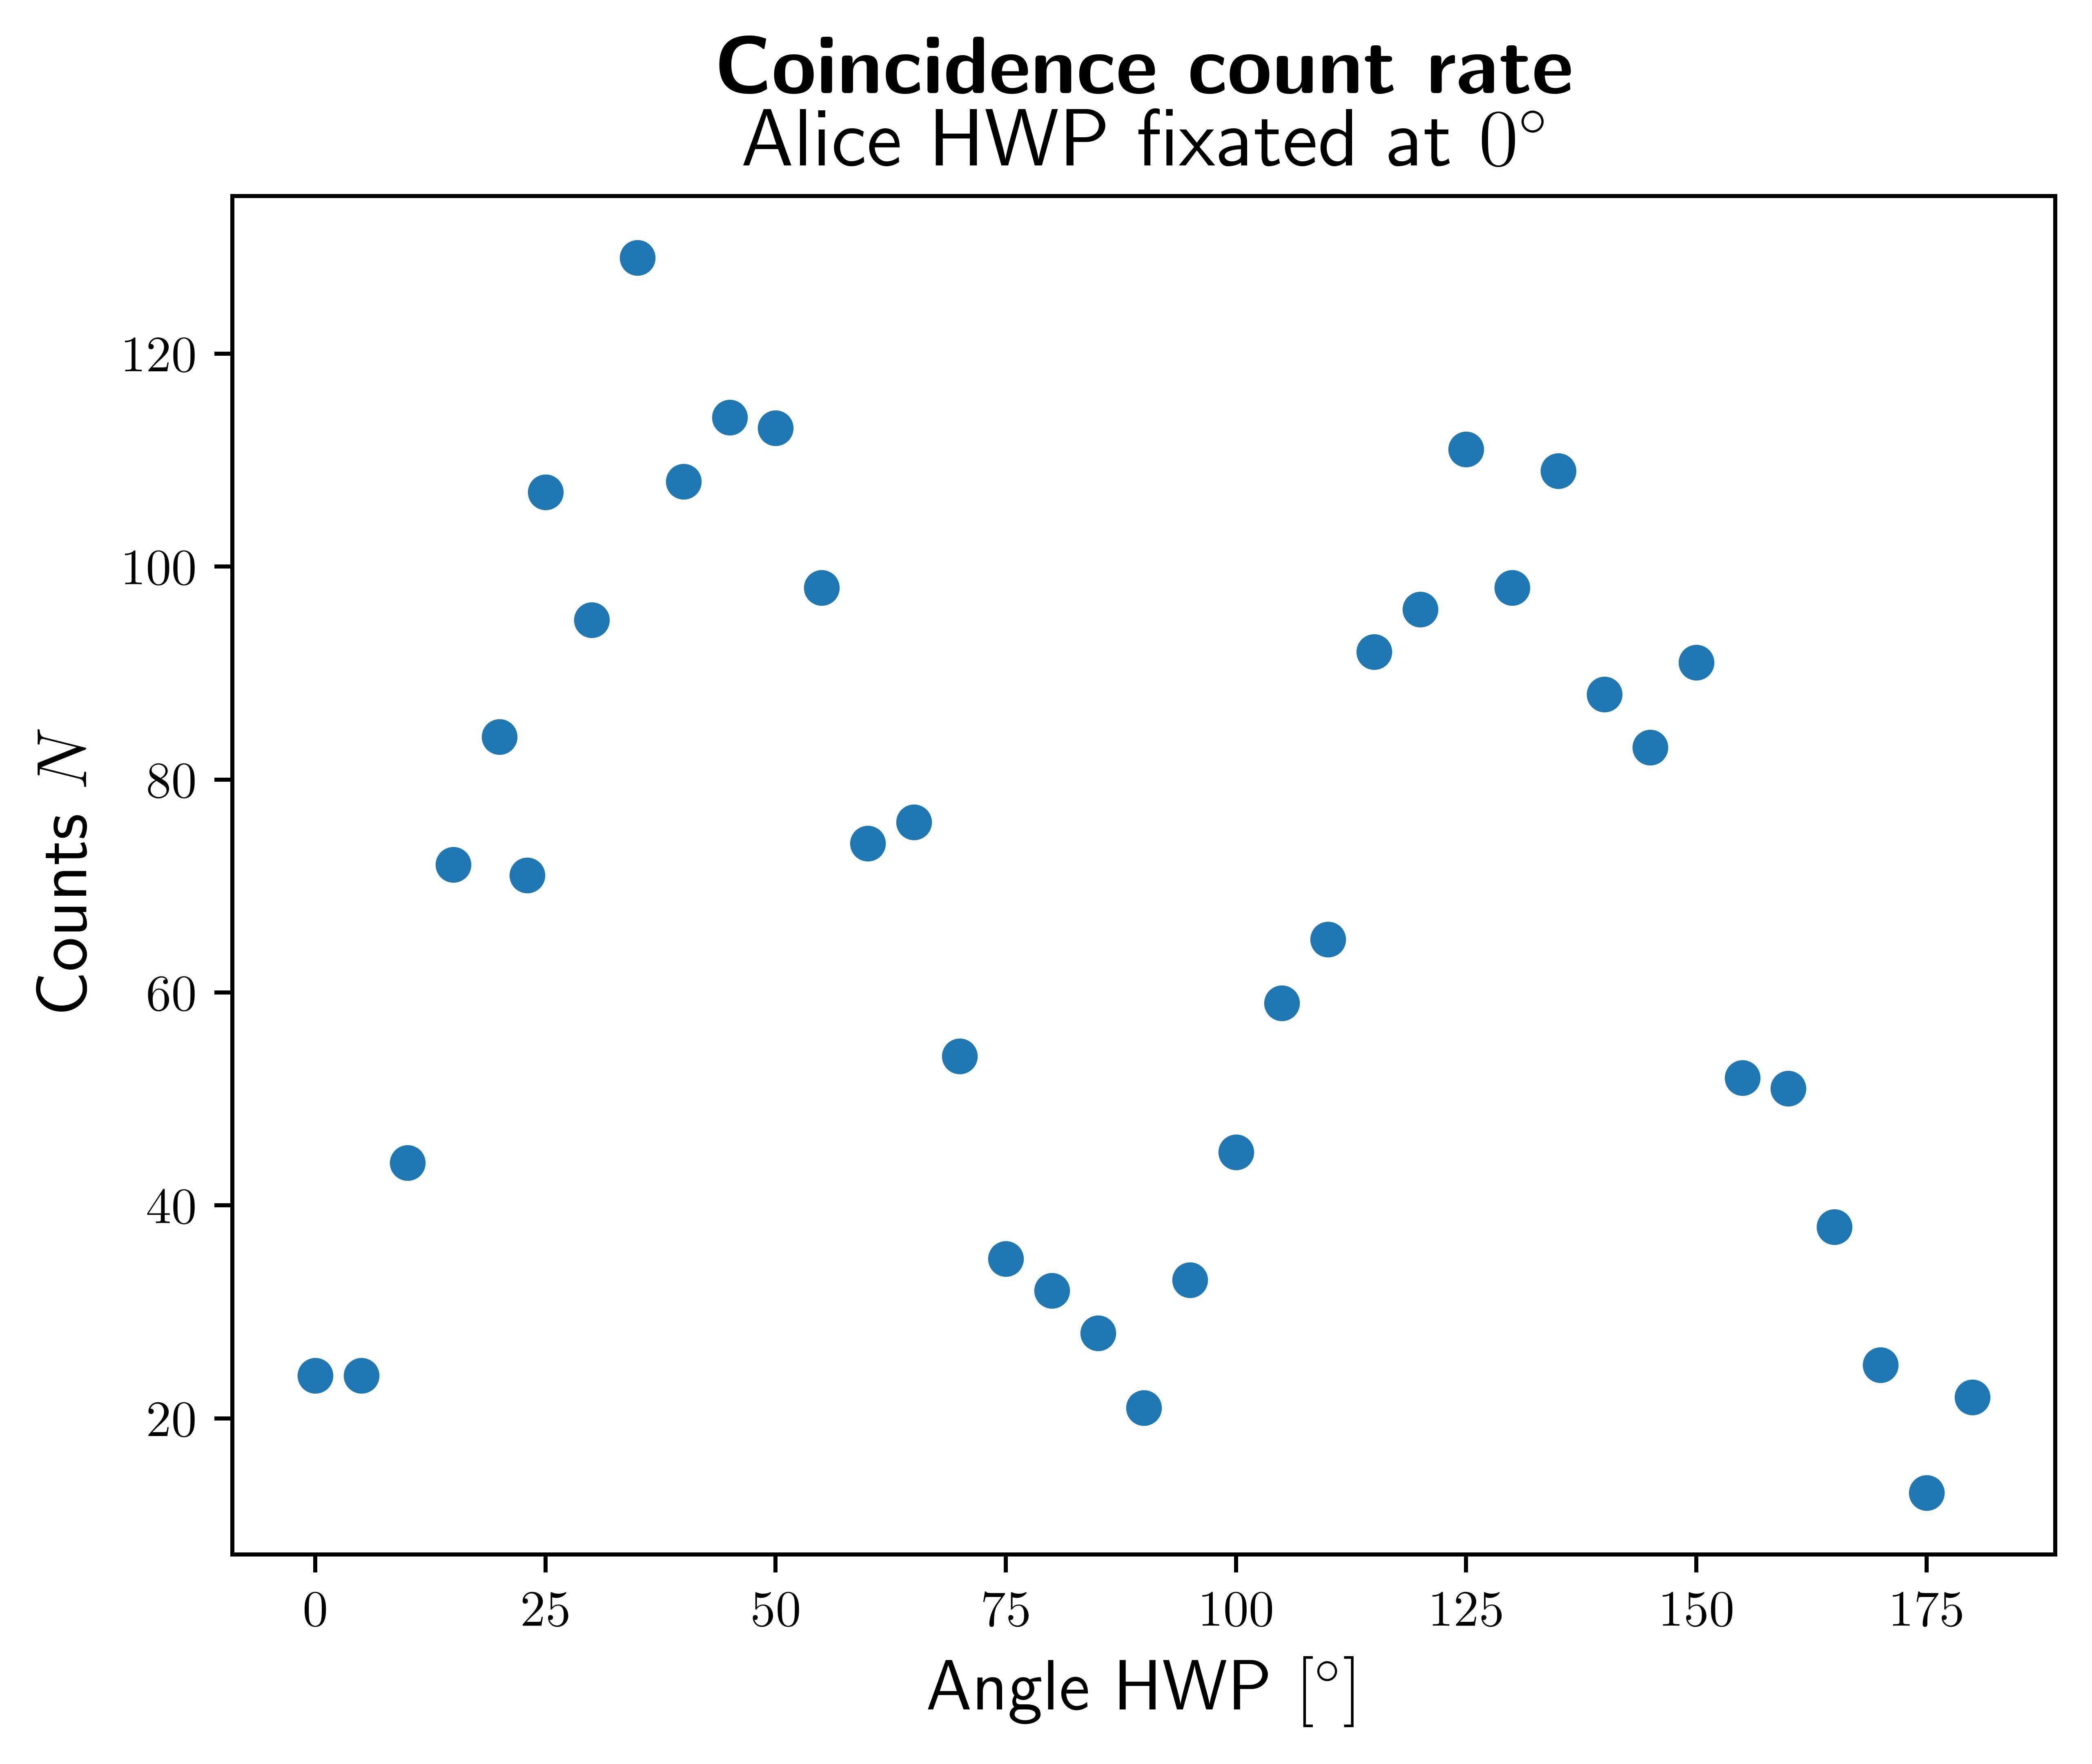
\includegraphics[width=\textwidth]{Koinzidenz/KoinzidenztählratenAliceFixiert0_90_A1B1.jpg  }
			\caption{Detektors A1B1}
			\label{fig:A1B1Alice0/90}
		\end{subfigure}
		\caption{
		    Koinzidenzzählraten der vier Detektorkombinationen für die Messreihe mit Alice Basis fixiert auf \(0/90 ^\circ \).
			Auffällig ist unter anderem der ungleichmäßige Verlauf, sowie die insgesamt geringere Zählraten der Detektoren A1B0 und A1B1.
		}
		\label{fig:KoinzidenzAlice0/90AlleDetektoren}
	\end{figure}



	\subsection{CHSH-Ungleichung}
	Nach der vorbereitenden Analyse der Zählraten wird im Folgenden die Verletzung der
	Bell'schen Ungleichung untersucht. Hier steht dabei nicht im Fokus die Korrektheit/Notwendigkeit
	der Quantenmechanik zu zeigen, statt dessen wird diese Verletzung als Maß genommen,
	das wir hier tatsächlich verschränkte Photonen messen, da dies Grundlegend für
	die im Ekert91 Protokoll verwendete Schlüsselgenerierung ist.
	Ohne Verschränkung wäre hier die Generierung nicht möglich, und bei vorheriger
	Zerstörung des verschränkten Zustandes, wäre die Sicherheit des Schlüssels zunichtegemacht.
	Für die Untersuchung wird dabei die CHSH Ungleichung
	\begin{equation}
	S = E(\vec{a}, \vec{b}) - E(\vec{a}, \vec{b}') + E(\vec{a}', \vec{b}) + E(\vec{a'}, \vec{b'})
	\end{equation}

	, eine umformulierte Variante der Bell'schen Ungleichung, wobei statt der Erwartungswerte
	die Korrelationsfunktion
	\begin{equation}
		C_{A,B} = \frac{N_{\alpha , \beta} + N_{\alpha^{\perp} , \beta^{\perp}} - N_{\alpha^{\perp} , \beta^{\perp}} - N_{\alpha , \beta}} {N_{\alpha , \beta} + N_{\alpha^{\perp} , \beta^{\perp}} + N_{\alpha^{\perp} , \beta^{\perp}} + N_{\alpha , \beta}}
		\label{eq:chshUngl}
	\end{equation}
	verwendet wird.
	\newline
	Bewegt sich dabei \(|S|\) in dem Intervall \(2 < |S| \leq 2\sqrt{2} \, (\approx 2.82)\),
	sind die gemessenen Photonen in einem verschränkten Zustand, sodass eine Schlüsselgenerierung möglich
	sei.

	Die verwendeten Werte für die verwendeten Basen \(\alpha\) und \(\beta\)
	sind dabei in \ref{tab:BellWinkelMaxVerletzung} gelistet.

	\begin{table}[H]
    	\caption{Winkeleinstellung für maximale Verletzung der Bell'schen Ungleichung}
    	\label{tab:BellWinkelMaxVerletzung}
        \begin{center}
			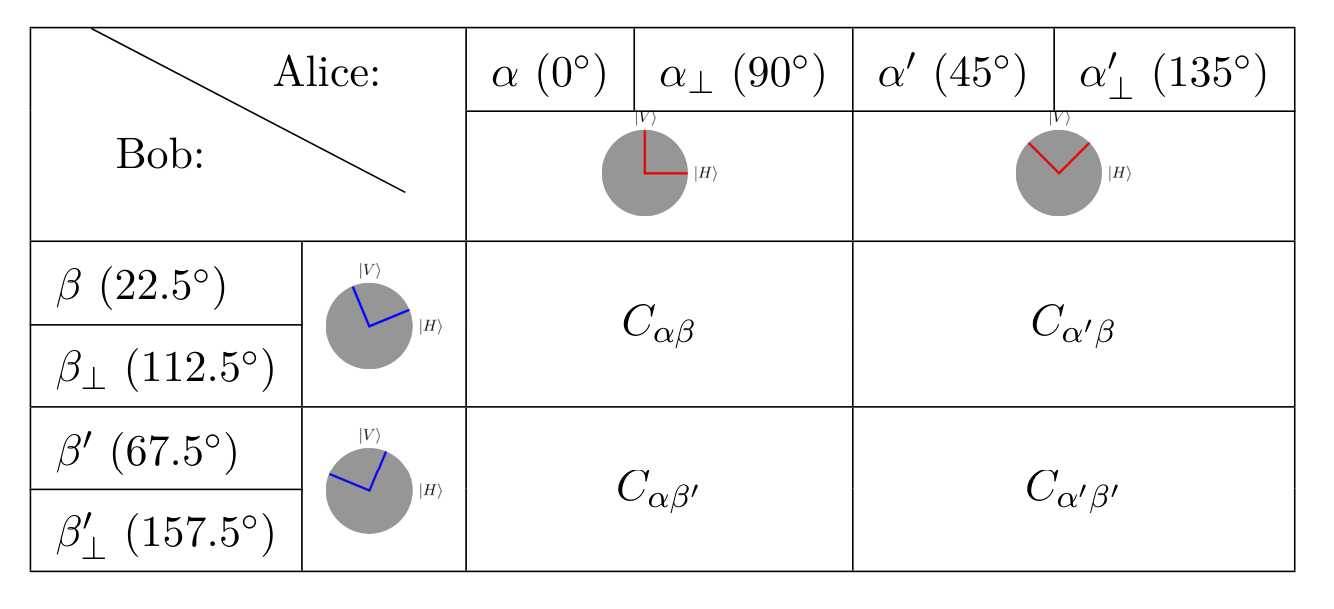
\includegraphics[width=0.95\textwidth]{Theorie/Screenshot From 2026-09-17 12-59-44.png}
		\end{center}
	\end{table}

	Die so ermittelten Werte für \(|S|\) sind in \ref{tab:SParam} einsehbar, und liegen mit
	\(2.24 \pm 0.05\) und \(2.25 \pm 0.05\) eindeutig über der Schwelle von \(2\).

	Hieraus lässt sich schließen, dass wir mit Verschränkten zuständen messen
	und der Aufbau, trotz der in den vorherigen Kapiteln erwähnten Problematiken,
	für die Schlüsselgenerierung verwendet werden kann.

	\begin{table}[H]
		\caption{S-Parameter}\label{tab:SParam}
		\begin{center}
			\begin{tabular}[c]{l|l|l}
				\hline
				\multicolumn{1}{c|}{\textbf{}} &
				\multicolumn{1}{c|}{\textbf{Messung 1}} &
				\multicolumn{1}{c}{\textbf{Messung 2}} \\
				\hline
				\(C_{AB}\) & \(-0.760 \pm 0.019\) & \(-0.752 \pm 0.020\) \\
				\(C_{AB}\) & \(\hspace{9.5} 0.561 \pm 0.025\) & \(\hspace{9.5}0.544 \pm 0.026\) \\
				\(C_{AB}\) & \(-0.401 \pm 0.028\) & \(-0.424 \pm 0.028\) \\
				\(C_{AB}\) & \(-0.518 \pm 0.025\) & \(-0.527 \pm 0.025\) \\
				\hline
				\(|\mathbf{S}|\) & \(\hspace{12.75} \mathbf{2.24\pm 0.05} \) & \(\hspace{12.75}\mathbf{2.25 \pm 0.05}\) \\
				\hline
			\end{tabular}
		\end{center}
	\end{table}

	\subsection{Schlüsselgenerierung und Spion}
	Im Folgenden sollte nun das Ekert-91 Protokoll verwendet werden, um einen Schlüssel zu
	generieren und diesen für die Kodierung einer Nachricht zu verwenden.
	\newline
	Hier kam es jedoch zu Problemen mit dem zugrunde legenden Python Skript, welches hierfür
	verwendet werden sollte:
	Für den Prozess der Generierung müssen viele konsekutive Messungen gemacht werden,
	welche bei Alice als auch bei Bob registriert werden müssen, jedoch kam es bei jedem Anlauf
	dazu, dass eine Seite eine Messung nicht in die Liste aufnahm, was damit einherging,
	dass keine weitere Messung mehr durchgeführt werden konnte.
	Nach dem fünften Anlauf und eineinhalb Stunden verstrichener Zeit,
	mussten wir leider einsehen, dass die Generierung so nicht möglich ist.
	\newline
	Aus diesem Grund wird im Folgenden der Prozess, wie er hätte ablaufen soll, erklärt
	und erläutert wie ein Spion zu erkennen wäre.
	\newline
	\newline
	Alice als auch Bob wählen für jede Messung zufällig eine der vier Basen aus Tabelle
	\ref{tab:BellWinkelMaxVerletzung}, über das Programm wird dann die verwendete Basis ausgetauscht.
	Bei gleicher verwendeter Basis wird dabei das Ergebnis behalten, anderenfalls wird das
	Ergebnis verworfen, dies wird so lange wiederholt, bis die gewünschte Schlüssellänge
	erreicht ist.
	Da nie Ergebnisse der Messungen übertragen wurden, ist der Schlüssel von
	außen nicht ersichtlich. Alice und Bob können jedoch aufgrund
	der verschränkten Zustände jeweils auf die Bitwerte des anderen Schließen bzw. haben jeweils den
	Inversen Schlüssel der anderen Partie.
	Zum Senden wird einfach der Schlüssel auf die Nachricht addiert und der Empfänger kann durch erneutes
	Addieren des eigenen Schlüssels und Invertieren der Bitfolge die Originalnachricht wieder erhalten.
	\newline
	\newline
	Ein Spion kann hierbei sehr einfach enttarnt werden, indem während der Schlüsselgenerierung
	auf die Verletzung der CHSH Ungleichung überprüft wird.
	\newline
	Dies ist dadurch gegeben, das ein Spion während der Schlüsselgenerierung die Bitwerte ermitteln muss
	und damit den Polarisationszustand der Photonen messen muss. Aufgrund des
	Non-Cloning-Theorems zerstört dies jedoch Zwangsläufig den verschränkten Zustand unwiderruflich,
	sodass bei Alice und Bob nur noch Photonen in klassischen Zuständen ankommen.
	Klassische Zustände können dabei nicht die CHSH Ungleichung verletzen und ergeben stets
	einen Wert für \(|S| \leq 2\).
\end{document}
